\section{Method}
By developing the unified representation for both data and domain knowledge, and utilizing ontological annotations, we can produce one RDF hypergraph, which serves as the basis for semantic data mining. Given this, the main research challenge is how to utilize the data and ontology together for semantic data mining. In this dissertation, we focus on one important data mining tasks, the {\em frequent pattern mining}, to showcase the utility of RDF hypergraphs.

\subsection{Frequent Pattern Mining}
\label{sec:association}
Frequent itemsets play an essential role in many data mining tasks that try to discover interesting relations between features in large databases. In the traditional sense, an itemset is called frequent if its support (number of times the itemset occur in the dataset) is no less than a given threshold. The original motivation for searching association rules came from the need to analyze supermarket customer behavior in terms of products that are often purchased together. However, it is evident that the measure of support essentially restrains pattern discovery to account for only directly associated items (\eg, products purchased together) while ignoring possible indirect associations. A prominent example of such indirect association was given by Swanson's land mark paper published in 1987~\cite{swanson87} that described the relationship between fish oil and Raynauld's syndrom through their mutual connections with certain changes in blood.

Such indirect associations can be best captured by graphs. In general, an object set endowed with pairwise relationships can be conceptually viewed as a graph in which vertices represent objects, and any two vertices that have some kind of relationship are joined together by an edge. In this sense the traditional measure of support evaluates the significance of a itemset by the number of direct edges (1-hop path) between item nodes. Extending this notion to allow paths with arbitrary lengths to be taken into account, we are able to evaluate the significance of an itemset in terms of the indirect connections among its nodes. From here on, we call the itemset associated by the indirect connection via multi-hop paths the \emph{semantically associated itemset}, or simply the \emph{semantic association}. In this chapter, We focus on describing graph-based algorithms to find semantically associated itemsets.

The term \emph{semantic association} conforms with the definition proposed by Sheth et al.~\cite{ShethEtal05JDBM} for semantic association between entities in an RDF graph. Specifically, they define the semantic association based on if there exists a sequence of interconnected links between two given entities. In our study of semantically associated itemsets in transaction data, the link between entities can be as simple as the `co-occurrence' relationship if more complicated relationships in ontologies are not concerned. Under Sheth et al's definition, the semantic association between transaction items $i_0$ and $i_n$ can be established by identifying a link of the form $i_0, P_c, i_1, P_c, \ldots , i_{n-1}, P_c, i_n$, in which $P_c$ denotes the property that connects two items (\eg, co-occurrence). Given this, the problem of finding meaningful semantic association becomes how to define a proper graph representation and effective analysis methods that can be carried out to evaluate the strength of semantic associations.

We first rule out simple graphs as the candidate model for discovering semantic associations due to the ambiguity and information loss. For illustrating this point of view, let us consider a relational table depicted in Figure~\ref{fig:hg_and_rg}(a). One can construct a simple undirected graph where the set of vertices is the set of relational attributes (column items) and an edge joins two vertices if the they co-occur in a tuple (as illustrated in Figure~\ref{fig:hg_and_rg}(b)). This graph is called \emph{Gaifman graph}~\cite{Hodkinson02finiteconformal} of a relational structure. The undirected graph can be further enriched by assigning to each edge a weight equal to the support of the 2-itemset consisting of vertices incident to the edge. Cliques (complete subgraphs) in the Gaifman graph, or \emph{Gaifman cliques} for short, are of particular interest because every tuple (ground atom) in data corresponds to a Gaifman clique. However, ambiguity arises as not all Gaifman cliques have matching tuple in the data. There exists cases where cliques are incidental in the sense that several relational ground atoms play together to induce a clique configuration in the Gaifman graph, but no ground atom covers the entire clique (e.g., the clique of $\{A,B,C,D\}$ in Figure~\ref{fig:hg_and_rg}(b) does not correspond to any tuple in the relational table). Further more, given the Gaifman graph we lose the information of how nodes are related. For example, if $A, B$ and $C$ are products purchased by a particular customer as indicated by a record in the transactional table, this information is no longer available in the graph

The RDF bipartite graph introduced in~\ref{sec:graph-rep-for-rdb} comes to remedy as it maximally preserves the semantics in the original table and contains no ambiguity. Plus it is able to represent ontologies in the same way so that analysis approaches on the RDF bipartite graph can systematically utilize information from both data and domain knowledge. Moreover, if a mining task does not involve the use of domain knowledge from ontologies, the RDF bipartite graph can be transformed to a more compact form that achieves better scalability. In the rest of this chapter, we describe in detail the methods for discovering semantically associated itemsets with and without the incorporation of ontologies respectively.

\subsection{Graph-based similarity}
Data mining algorithms rely on the notion of similarity between data points to make meaningful inferences. When data is in $\mathbb{R}^d$, the standard similarity measure is the Euclidean distance. When data has an explicit link structure, shortest path distance is commonly used. However, neither of these measures incorporates the intuition that two data points are similar to each other if they are connected by a high density region. This latter concept of similarity measure has been shown in experiments to lead to significant improvement in a number of learning tasks, see, for example, (Blum \& Chawla, 2001; Corduneanu \& Jaakkola, 2003; Bous-quet et al., 2004)~\cite{}.

Take the simple graph in Fig.~\ref{fig:graphcomp}(B) for example, suppose given a task of friend recommendation based on the information in this graph, the interesting question is whether $c$ or $e$ is a better choice of recommendation to $a$. To answer this question, it is natural to compare the similarity measures $s(a, c)$ and $s(a, e)$. In a rough sense, on can identify in the hypergraph representation that there are two paths between $a$ and $c$ (the formal definition for paths in hypergraphs will be given in Section~\ref{sec:rw_hyper}), while only one between $a$ and $e$. It's intuitive to conclude that $a$ and $c$ are more similar, or closer, than $a$ and $e$. This gives us a hint that meaningful similarity measures on the graph should satisfy the following intuitions:
\begin{enumerate}
\item The more paths connecting two nodes, the closer they are.
\item The shorter the paths, the closer they are.
\end{enumerate}
In other words, the more ``short" connections between two given nodes, the more similar those nodes are.
To this end, we propose to employ the following quantities as the candidate similarity measure since both of them have the desired property. They are, namely, the \emph{commute time distance} based similarity measure from the random walk model on hypergraph, and the inner product similarity based on the \emph{pseudoinverse of the hypergraph Laplacian}.
Several measures derived from random walk on graphs have been shown to possess such desired property. In the following example, we quantitatively show the property of commute time distance, which characterizes the expected number of steps to take a round trip between a starting node and a target node.

\begin{figure}[tbh]
\centering
\begin{minipage}[c]{\textwidth}\centering
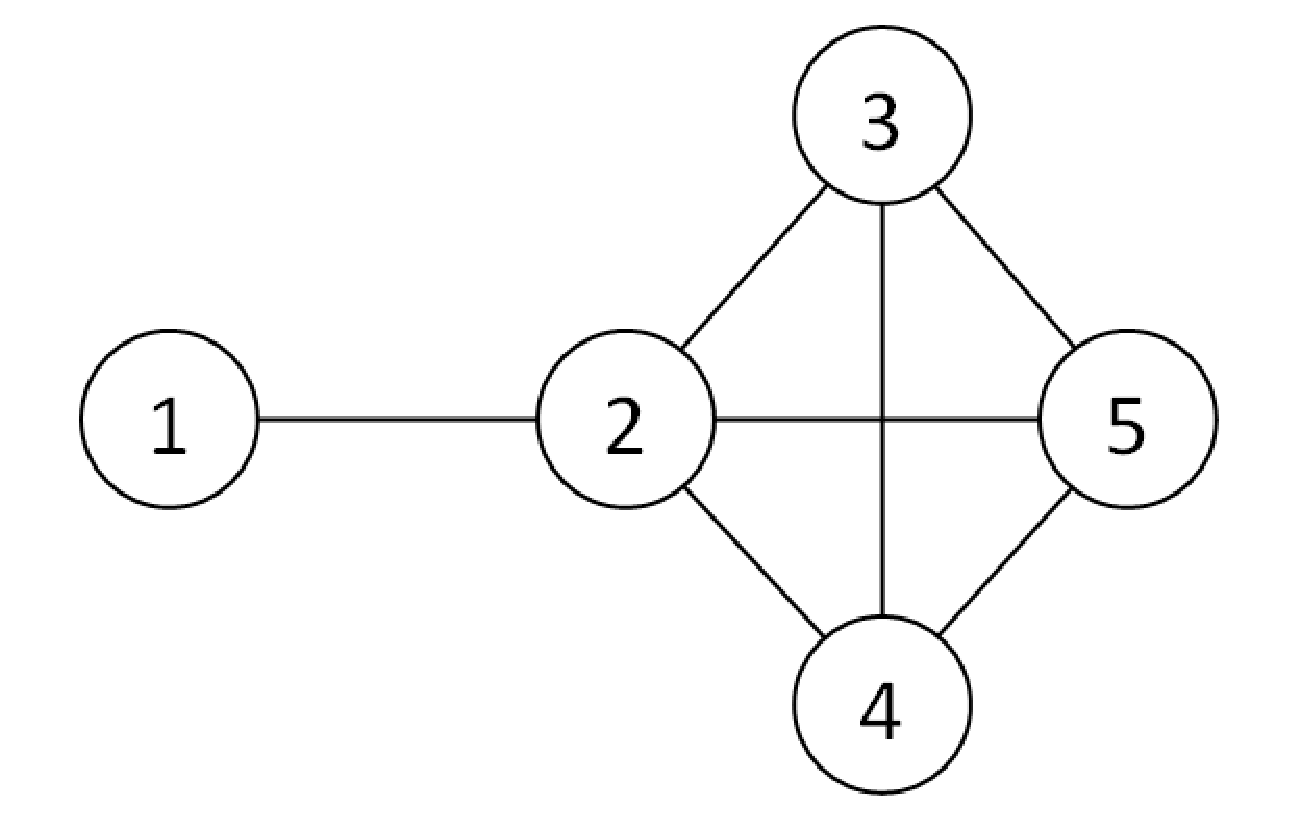
\includegraphics[width=.4\textwidth]{fig/comm-dist-demo.eps}
\end{minipage}
\hfill
\begin{minipage}[c]{\textwidth}\centering
\begin{tabular}{r|r|r|r|r|r || r|r|r|r|r}
\hline\hline
\multicolumn{6}{c||}{Euclidian Distance}	&	\multicolumn{5}{c}{Commute Distance}		\\
\hline\hline							
Index	&	1	&	2	&	3	&	4	&	5	&	1	&	2	&	3	&	4	&	5	\\
\hline
1	&	0	&	1	&	1.85	&	1.85	&	2.41	&	0	&	12.83	&	19.79	&	19.79	&	20.34	\\
\hline
2	&	1	&	0	&	1	&	1	&	1.41	&	12.83	&	0	&	6.96	&	6.96	&	7.51	\\
\hline
3	&	1.85	&	1	&	0	&	1.41	&	1	&	19.79	&	6.96	&	0	&	7.51	&	6.96	\\
\hline
4	&	1.85	&	1	&	1.41	&	0	&	1	&	19.79	&	6.96	&	7.51	&	0	&	6.96	\\
\hline
5	&	2.41	&	1.41	&	1	&	1	&	0	&	20.34	&	7.51	&	6.96	&	6.96	&	0	\\
\hline\hline
\end{tabular}
\end{minipage}
\caption{\label{fig:cd-demo} A Comparison between the Euclidean distance and the commute time distance.}
\end{figure}

Figure~\ref{fig:cd-demo} shows a graph of five nodes with a specific edge configuration (the so called ``lollipop graph''). The Euclidean distance between each pair of nodes are shown in the left-hand side of the corresponding table above and the respective commute time distance are shown on the righ-hand side. It can be seen that node 1 and node 3 are equally close to node 2 in terms of their Euclidean distances. However, node 2 and 3 are considered much closer under commute time distance because they are within a much more densely connected subgraph. This shows that, unlike Euclidean distance and shortest path distance, commute distance between two nodes captures both the length of paths between them and their local neighborhood densities. We believe such property makes the commute time distance a suitable measure for graph-based data mining algorithms. We also explore other random walk-based measures including the pseudoinverse of the Laplacian matrix and the stationary probability that are closely related to commute time distance. In the following, we first describe random walk on simple graph and then introduce the extension to hypergraph. The details of hypergraph-based similarity measures are described in the subsequent sections.
%These methods are described in detail in the following sections and trade-offs between them are studied.

\subsubsection{Random Walk}
\textbf{Random Walk on Simple Graph}
Given a graph and a starting point we select a neighbor of it at random and move to this neighbor then we select a neighbor of this point at random and move to it etc. The random sequence of points selected this way is a random walk on the graph. In other words, a random walker can jump from vertex to vertex and each vertex therefore represents a state of the Markov chain. The average first-passage time $m(k|i)$~\cite{randomwalks} is the average number of steps needed by a random walker for reaching state $k$ for the first time, when starting from state $i$. The symmetrized quantity $n(i,j)=m(j|i)+m(i|j)$ called the average commute time~\cite{randomwalks}, provides a distance measure between any pair of states. The fact that this quantity is indeed a distance on a graph was proved independently by Klein and Randic~\cite{Klein} and Gobel and Jagers~\cite{Gobel}.

The Laplacian matrix $\mathbf{L}$ of a graph is widely used for finding many properties of the graphs in spectral graph theory. Given node degree matrix $\mathbf{D}$ and graph adjacency matrix $\mathbf{A}$, the Laplacian matrix of the graph is defined as $\mathbf{L}=\mathbf{D}-\mathbf{A}$. The normalized Laplacian is given by $\mathbf{L}_N=\mathbf{I}-\mathbf{D}^{-1/2}\mathbf{A}\mathbf{D}^{-1/2}$, where $\mathbf{I}$ is the identity matrix. The average commute time $n(i,j)$ can be computed in closed form from the Moore-Penrose pseudoinverse of $\mathbf{L}$~\cite{pseudo}, denoted by $\mathbf{L}^+$.

Various quantities derived from random walk on graph has been used in a number of applications. Fouss et al.~\cite{Fouss06random-walkcomputation} compared twelve scoring algorithms based on graph representation of the database to perform collaborative movie recommendation. Pan et al.~\cite{Pan} developed a similarity measure based on random walk steady state probability to discover correlation between multimedia objects containing data of various modalities. Yen et al.~\cite{Yen05clusteringusing} introduced a new k-means clustering algorithm utilizing the random walk average commute time distance. Zhou et al.~\cite{Zhou:2009:GCB:1687627.1687709} presented a unified framework based on neighborhood random walk to integrate structural and attribute similarities for graph clustering.

\textbf{Random Walk on Hypergraph}
\label{sec:rw_hyper}
We can associate each hypergraph with a natural random walk which has the transition rule as described in~\cite{Zhou06learningwith}. Given the current position $u \in V$; first choose a hyperedge $e$ over all hyperedges incident with $u$ with the probability proportional to $w(e)$; and then choose a vertex $v \in e$ uniformly at random. Obviously, it generalizes the natural random walk defined on simple graphs. Let $\mathbf{P}$ denote the transition probability matrix of this hypergraph random walk.
Then each entry of $\mathbf{P}$ is
\[
p(u,v) = \sum_{e\in E}{w(e)\frac{h(u,e)}{d(u)}\frac{h(v,e)}{\delta(e)}}\, .
\]
In matrix notation, $\mathbf{P}=\mathbf{D}_v^{-1}\mathbf{HWD}_e^{-1}\mathbf{H}^T$.
Zhou et al.~\cite{Zhou06learningwith} define the following normalized hypergraph Laplacian $\mathcal{L}$ based on the random walk model:
\begin{align}
\mathcal{L}=\mathbf{I}-\mathbf{\Theta},   ~\mathrm{where}~ \mathbf{\Theta}=\mathbf{D}_v^{-\frac12}\mathbf{HWD}_e^{-1}\mathbf{H}^T\mathbf{D}_v^{-\frac12} \label{eq:normalizedHyperL}.
\end{align}

\section{Mining Semantically Associated Itemsets without Ontologies}
In this section, we present our study for discovering semantically associated itemsets based on hypergraph without incorporating domain knowledge in ontologies. The goal of this study is to show that, using graph based formalism, we can obtain interesting patterns that are unable to be captured by traditional methods.

If a mining task does not involve the usage of ontologies and focuses only on data in tables, we can use an alternative hypergraph representation that is more compact than the RDF bipartite graph to model the data. The process to generate such hypergraph is called \emph{RDF hypergraph coarsening} as described in Definition~\ref{def:hg-coarsen}.

\subsection{RDF Hypergraph Coarsening}

\begin{figure}[tbh]
\centering
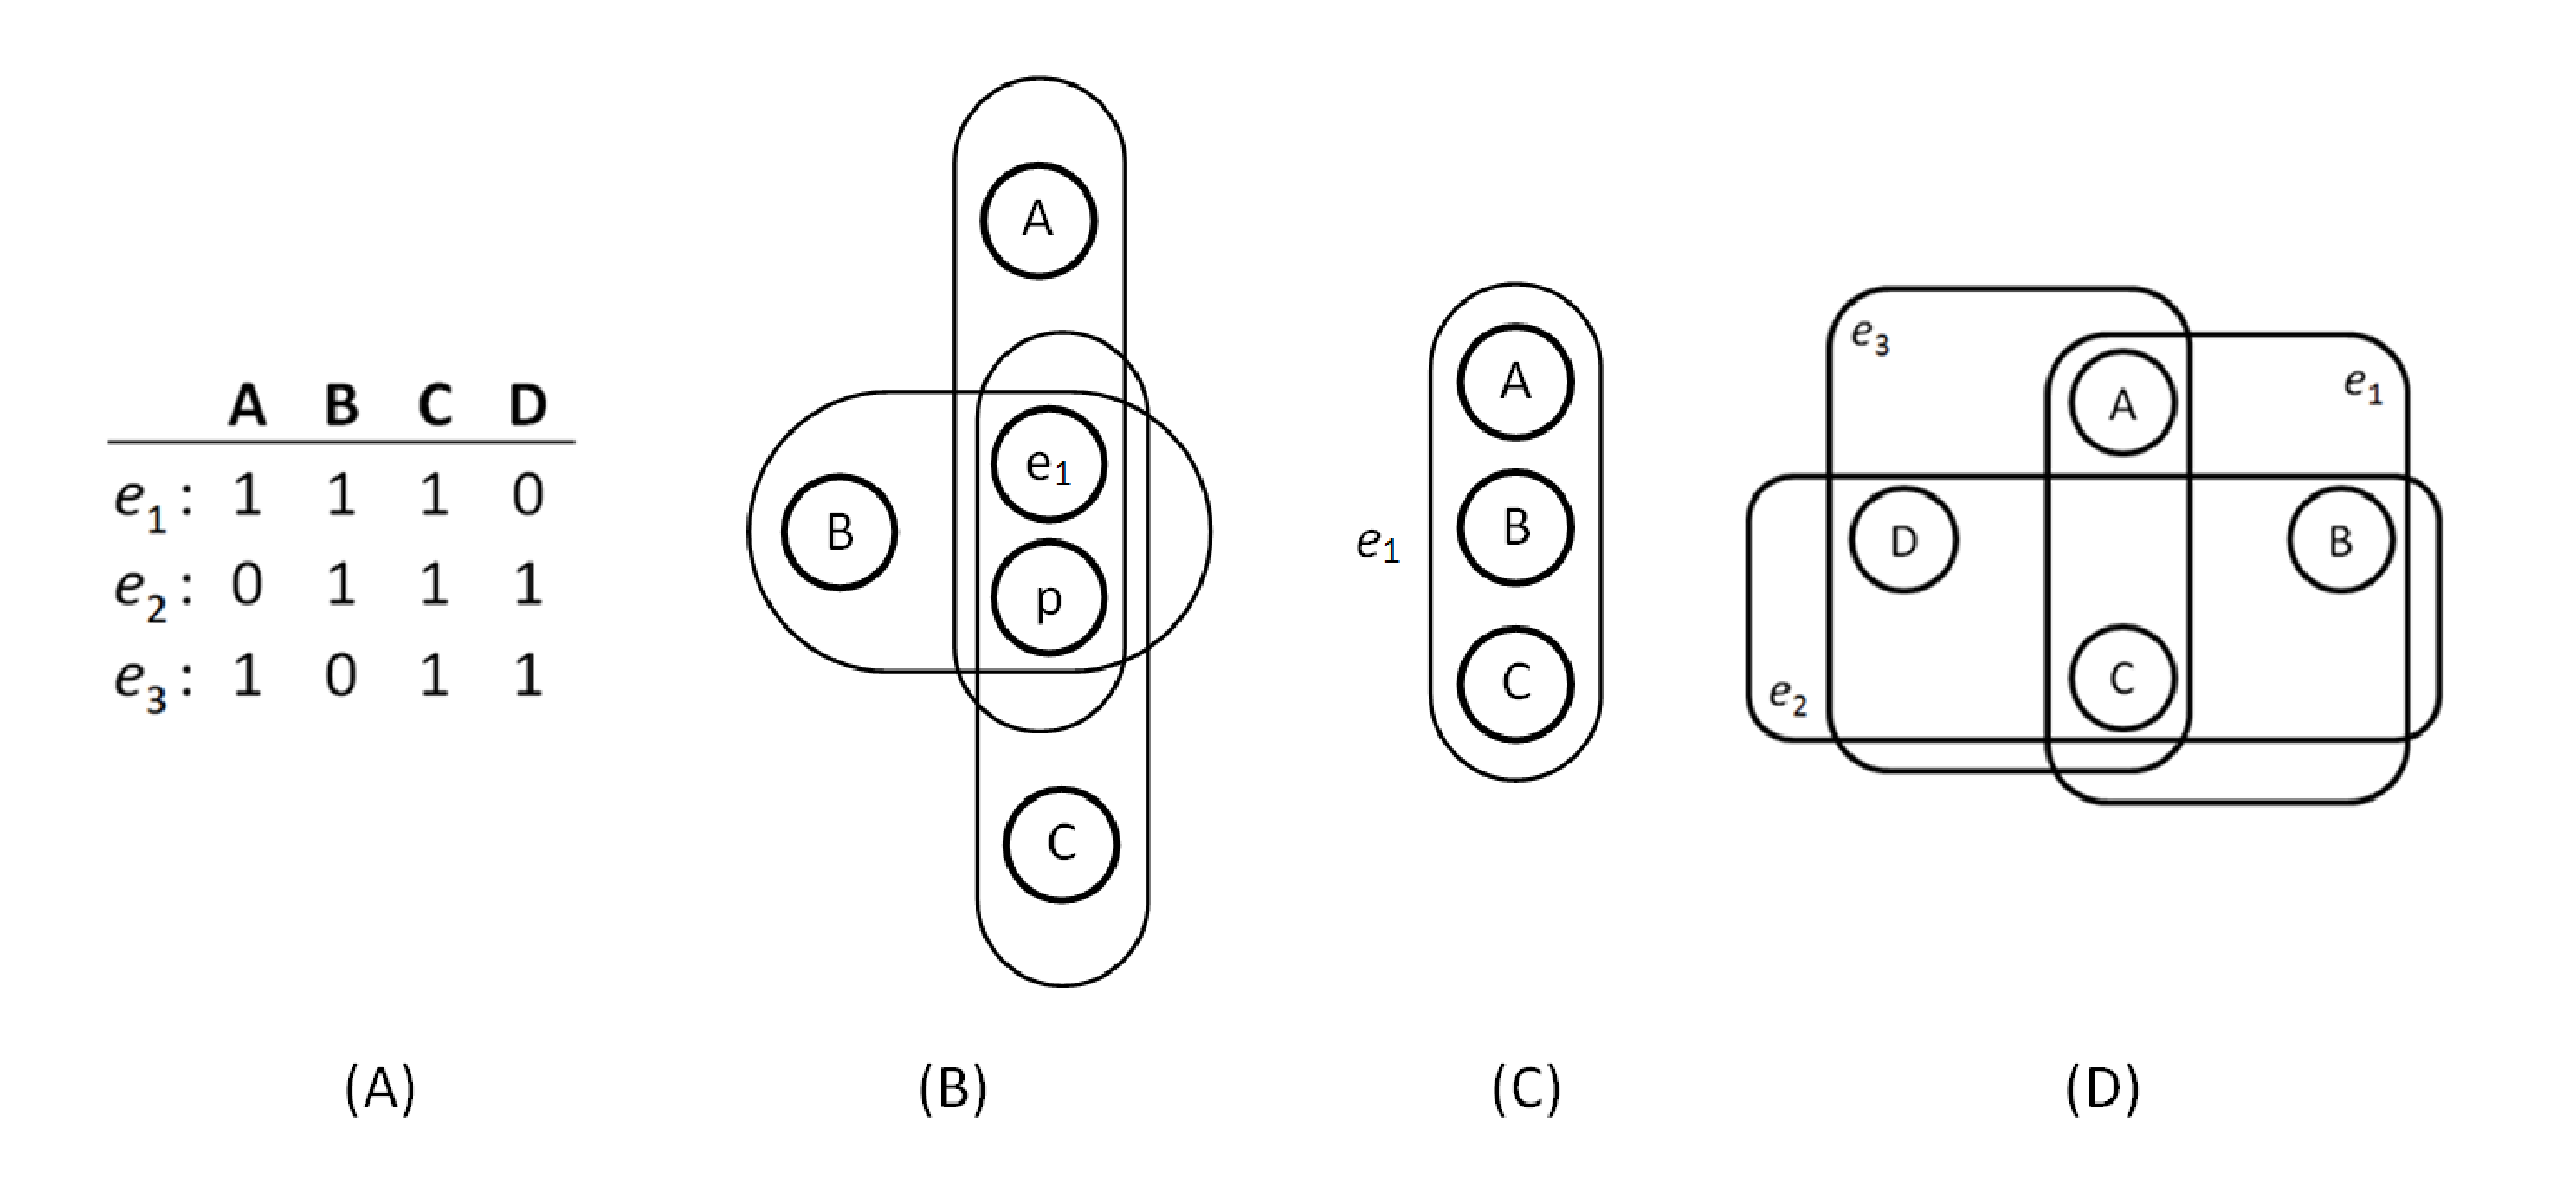
\includegraphics[width=\textwidth]{fig/hypergraph-coarsening.eps}
\caption{\label{fig:hypergraph-coarsening} An example hypergraph coarsening process.}
\end{figure}

\begin{mydef}[\textbf{RDF hypergraph coarsening}]
\label{def:hg-coarsen}
RDF hypergraph coarsening is the process of computing a compact form given an input RDF hypergraph for a relational table by merging vertices into larger groups and removing less significant vertices. The choice of vertices is pertinent to the specific mining tasks. Note that RDF hypergraph is 3-uniform and in the case of RDF hypergraph for relation tables, each hyperedge has three nodes corresponding to the RDF statement of the form \texttt{<row>, <p>, <column>}. The \texttt{<p>} node is the auxiliary predicate denoting the context-dependent semantic relationship between the row and column nodes (\eg, such as that can be as general as \texttt{<mentions>}), and since it is incident to all RDF hyperedges it is first removed in the coarsening process as it bears the least amount of information. Next, if the mining task focuses on discovering patterns among column nodes (\eg, frequent pattern mining), we can merge column nodes that coincide with the same row nodes into a new hyperedge and subsequently remove the row node, and vice versa for mining tasks focusing on row nodes.
\end{mydef}

\begin{myexp}[\textbf{Generation of a column-wise hypergraph for a relational table}]
\label{column-wise-hg}
Figure~\ref{fig:hypergraph-coarsening} (A) shows a sample relational table. Using the method described in Example~\ref{exp:repBinRDB} we can represent this binary-valued table to an RDF hypergraph as is shown in Figure~\ref{fig:hypergraph-coarsening} (B), which demonstrates three hyperedges corresponding to the first row in the table created by transforming the row into three RDF statements, i.e., \texttt{<$e_1$, p, A>, <$e_1$, p, B>}, and \texttt{<$e_1$, p, C>}. Figure~\ref{fig:hypergraph-coarsening} (C) illustrates the coarsened hypergraph according to Definition~\ref{def:hg-coarsen}. Supposing we are interested in discovering relationship between column nodes \texttt{A, B} and \texttt{C} in a frequent pattern mining task, we can remove the nodes \texttt{$e_1$} and \texttt{p} that are commonly incident to all the three hyperedges, and then merge nodes \texttt{A, B} and \texttt{C} to form a single hyperedge. Figure~\ref{fig:hypergraph-coarsening} (D) shows the resulting coarsened hypergraph for the relational table in Figure~\ref{fig:hypergraph-coarsening} (A).
\end{myexp}

Given the method for RDF hypergraph coarsening, we propose to construct a coarsed hypergraph for the relational table in the scenario where ontologies are not included. The relational attributes constitute the universe of vertices in the hypergraph. Based on this hypergraph, our approach for mining semantically associated itemsets starts by first generating 2-itemsets. A 2-itemset $\langle i,j \rangle$ is considered semantically associated if the hypergraph-based similarity measure $s(i,j)$ exceeds some threshold. In the following, we describe two similarity measures $s_{CT}$ and $s_{L+}$ based on, respectively, the average commute time distance on hypergraph and the inner-product-based representation of the pseudoinverse of Hypergraph Laplacian. Given discovered semantically associated 2-itemsets, we propose a hypergraph expansion method along with two search strategies, namely, the clique and connected component search, in the resulting graph for finding semantically associated $k$-itemsets ($k>2$).
\begin{figure*}[tbh]
\begin{center}
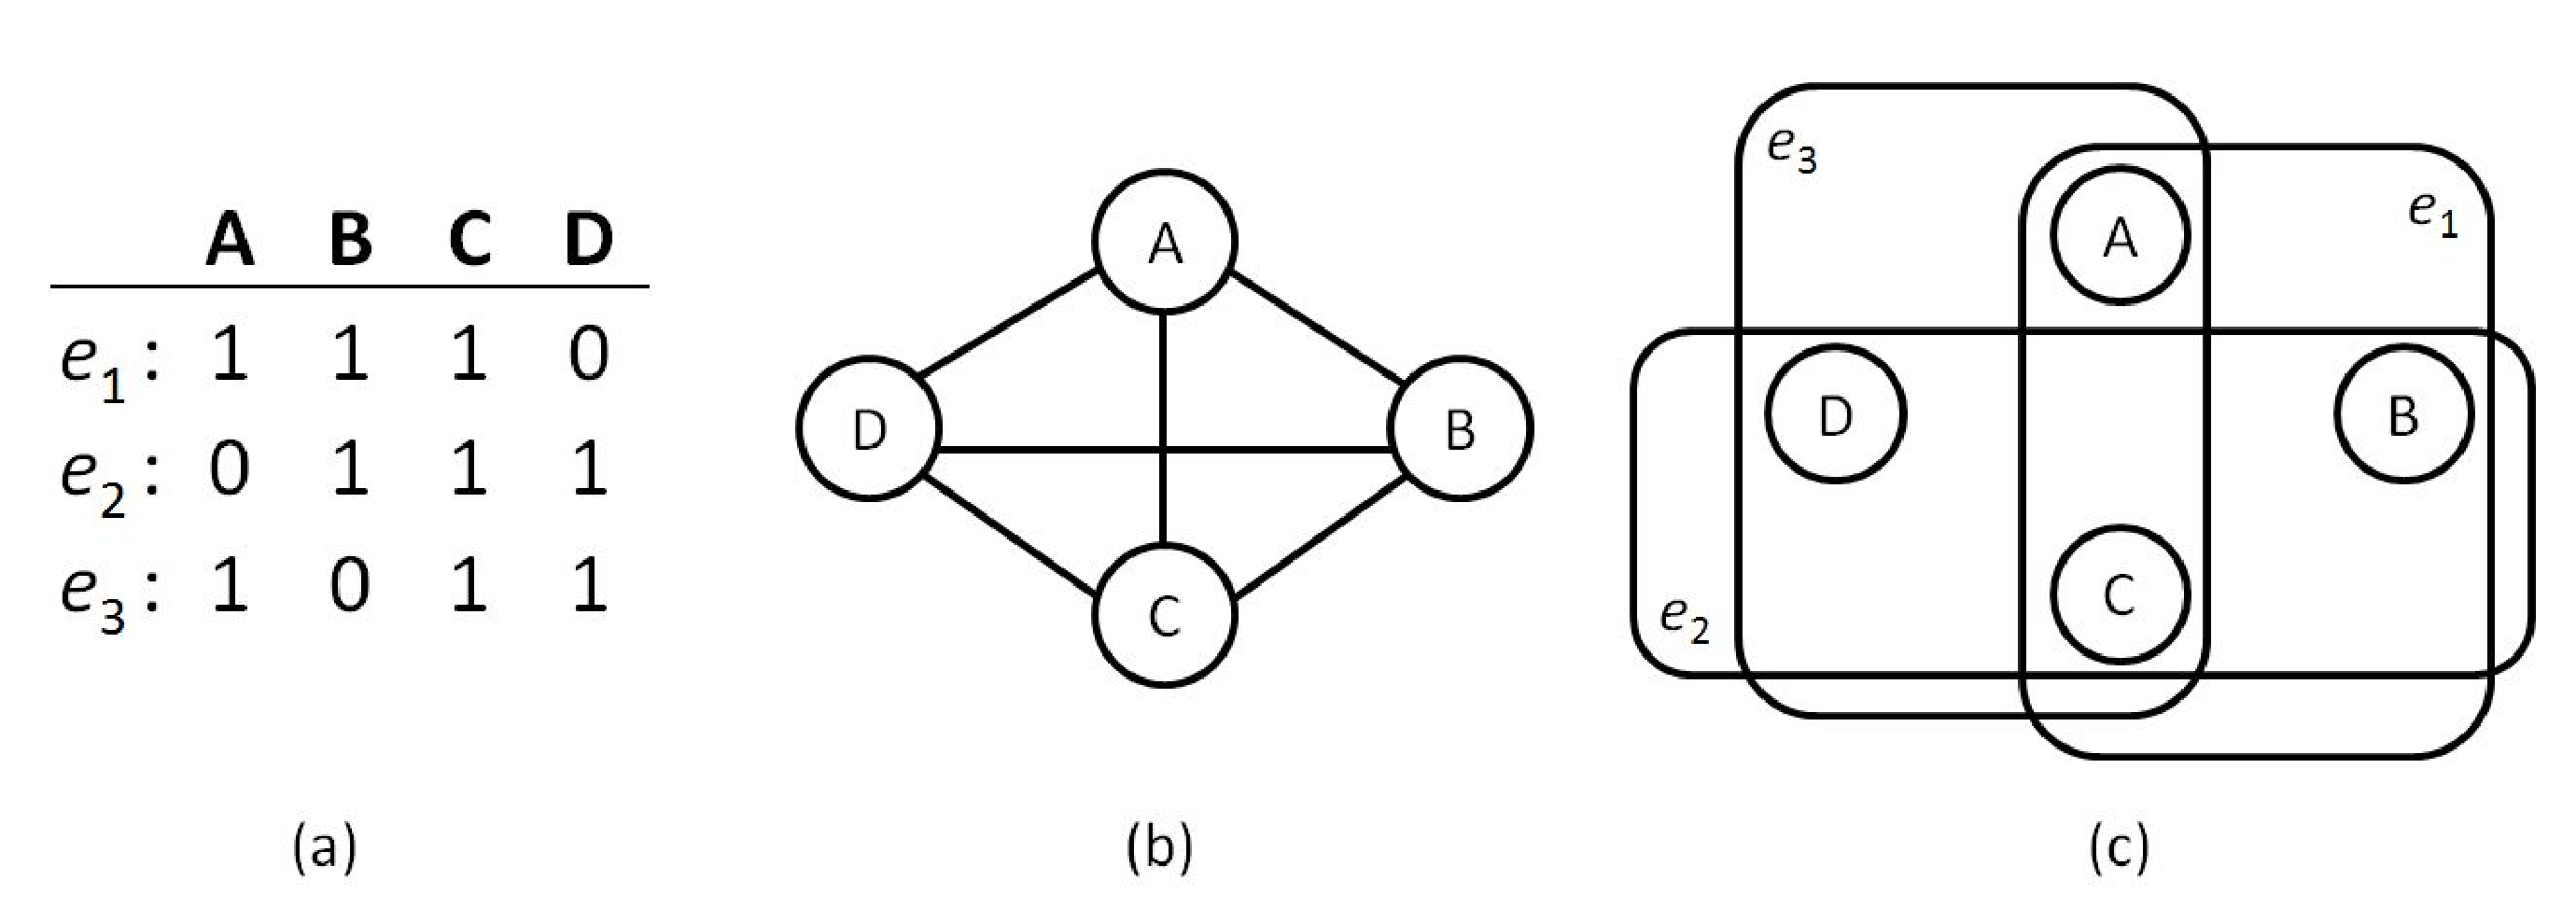
\includegraphics[width=.8\textwidth]{fig/hg_and_rg1.eps}
\end{center}
\caption[The simple graph vs. hypergraph for representing a relational table.]{\label{fig:hg_and_rg} (a) an example transaction table; (b) the Gaifman graph representation of the table; (c) The hypergraph representation of the table}
\end{figure*}

\subsubsection{Methods for Generating 2-itemsets}
In the following we describe two similarity measures that define the strength of bond between a pair of semantically associated items.

\textbf{Average Commute Time Similarity $s_{CT}$}\\
To compute commute-time distance between vertices in a hypergraph, we need to first define the combinatory hypergraph Laplacian $\mathbf{L}$.
It follows from Zhou et al's formalism of normalized hypergraph Laplacian in Equation~\ref{eq:normalizedHyperL} that:
\begin{equation}
\mathbf{L}=\mathbf{D}^{1/2}\mathcal{L}\mathbf{D}^{-1/2}=\mathbf{D}_v-\mathbf{HWD}_e^{-1}\mathbf{H}^T \label{eq:combinatoryHyperL}
\end{equation}

The average commute time $n(i,j)$ on simple graph can be computed in closed form from the Moore-Penrose pseudoinverse of $\mathbf{L}$ ~\cite{pseudo}, denoted by $\mathbf{L}^+$ with elements $l_{ij}^+=[\mathbf{L}^+]_{ij}$. It can be shown that $n(i,j)$ on hypergraph can be calculated in the same manner. The pseudoinverse $\mathbf{L}^+$ is given by the following equation:
\begin{equation}
\mathbf{L}^+=(\mathbf{L} -\mathbf{ee}^T/n)^{-1} + \mathbf{ee}^T/n, \label{eq:pL}
\end{equation}
where $\mathbf{e}$ is a column vector made of 1s (i.e., $\mathbf{e}=[1,1,\ldots,1]^T$). The formula for the computation of $n(i,j)$ takes the form of the following equation:
\begin{equation}
n(i,j)=V_G(l_{ii}^+ + l_{jj}^+ - 2l_{ij}^+) \label{eq:CT},
\end{equation}
where $V_G = tr(\mathbf{D}_v)$ is the volume of the hypergraph. If we define $\mathbf{e}_i$ as the $i$th column of $\mathbf{I}$ (i.e.,
$
\mathbf{e}_i=[\stackbin[1]{}{0}, \ldots, \stackbin[i-1]{}{0}, \stackbin[i]{}{1},$
$ \stackbin[i+1]{}{0}, \ldots, \stackbin[n]{}{0}]^T
$),
Equation~\ref{eq:CT} can be transformed to:
\begin{align}
n(i,j)=V_G(\mathbf{e}_i-\mathbf{e}_j)^T\mathbf{L}^+(\mathbf{e}_i-\mathbf{e}_j), \label{eq:CT2}
\end{align}
Since $n(i,j)$ is a distance, it is straightforward to convert it to a similarity measure $s_{CT}(i,j)$ by normalize it to unit range and subtract from 1.

\textbf{Pseudoinverse-based Inner-Product Similarity $s_{L+}$}\\
Equation \ref{eq:CT2} can be mapped into a new Euclidean space that preserves the commute time distance:
\begin{align}
\notag n(i,j)&=V_G(\mathbf{e}_i-\mathbf{e}_j)^T\mathbf{L}^+(\mathbf{e}_i-\mathbf{e}_j)\\
\notag &=V_G(\mathbf{x}_i'-\mathbf{x}_j')^T(\mathbf{x}_i'-\mathbf{x}_j')\\
&=V_G\|\mathbf{x}_i'-\mathbf{x}_j'\|^2, \label{eq:ECTD}
\end{align}
where $\mathbf{x}_i'=\mathbf{\Lambda}^{1/2}\mathbf{U}^T\mathbf{e}_i$, $\mathbf{U}$ is an orthonormal matrix made of eigenvectors of $\mathbf{L}^+$ (ordered in decreasing order of corresponding eigenvalue $\lambda_k$) and $\mathbf{\Lambda}=\mathbf{Diag}(\lambda_k)$. In this way, the transformed node vectors $\mathbf{x}_i'$ are exactly separated in the new $n$-dimensional Euclidean space.
From this definition, it follows that $\mathbf{L}^+ $ is the matrix containing inner products of the transformed vectors $\mathbf{x}_i'$ as shown below:
\begin{align}
\notag \mathbf{x}_i'^T\mathbf{x}_j'&=(\mathbf{\Lambda}_i^{1/2}\mathbf{x}_i)^T\mathbf{\Lambda}_j^{1/2}\mathbf{x}_j=\mathbf{x}_i^T\mathbf{\Lambda}\mathbf{x}_j\\
&=\mathbf{e}_i^T\mathbf{U\Lambda U}^T\mathbf{e}_j=\mathbf{e}_i^T\mathbf{L}^+\mathbf{e}_j=l_{ij}^+.
\end{align}
Therefore, $\mathbf{L}^+$ can be considered as a similarity matrix for the nodes---that is
\begin{equation}
s_{L^+}(i,j)=l_{ij}^+ \, . \label{eq:sim_L+}
\end{equation}
The inner-product-based similarity measures are well-studied for the vector-space model of information retrieval. It has been shown that when computing proximities between documents, inner-product-based measures outperform Euclidean distances~\cite{IR}.

\subsubsection{Effective Computation}
\label{sec:eff_comp}
In high dimensional data sets, the computations of the Hypergraph Laplacian and the pseudoinverse becomes intractable. We discuss two approaches to mitigate this scalability problem.

To compute Hypergraph Laplacian $\mathbf{L}$ in Equation \ref{eq:combinatoryHyperL} requires multiplication of hypergraph incidence matrices $\mathbf{H}$ and its transpose $\mathbf{H}^T$. Since $\mathbf{H}$ grows in proportion to the size of underlying transaction data (each node corresponds to a column and each hyperedge corresponds to a row), it eventually becomes unable to fit in memory when the size exceeding a certain amount. In this case the computation can still be carried out using a block partitioned matrix product by performing operations only on the submatrices of tractable sizes. Owing to the fact that, in most cases, $|V|$ is much smaller than $|E|$, $\mathbf{H}$ can then be partitioned into $s$ vertical stripes and the square matrix $\mathbf{D}_e$ into $s$ diagonal blocks. The multiplication in Equation \ref{eq:combinatoryHyperL} can be calculated by $\mathbf{HD}_e^{-1}\mathbf{H}^T=\sum_{\gamma=1}^s{\mathbf{H}_\gamma\mathbf{D}_{e\gamma}^{-1}\mathbf{H}_\gamma^T}$. Note that $\mathbf{H}$ is sparse in many applications. This property can be exploited to gain high performance and due to its importance much effort has been devoted to the study resulting a number of libraries and routines from which we can leverage.

As the number of nodes grows, to compute pseudoinverse in closed form using Equation \ref{eq:pL} also becomes intractable. A procedure based on Cholesky factorization to compute $\mathbf{L}^+$ for large sparse matrices~\cite{matrix} is proved useful. It allows to compute $\mathbf{L}^+$ in a column-by-column manner. In particular, the procedure involves the following steps for computing the $i$th column of $\mathbf{L}^+$:
\begin{enumerate}
\item Compute the projection $\mathbf{y}_i$ of base vector $\mathbf{e}_i$ on the column space of $\mathbf{L}$.
\item Find a solution $l_i^{*+}$ of the linear system $\mathbf{Ll}=\mathbf{y}_i$.
\item Project $l_i^{*+}$ on the row space of $\mathbf{L}$ to get $l_i^+$.
\end{enumerate}
Since $\mathbf{L}$ is symmetric, its row space is the same as column space. The projection in step 1 and 2 can be represented by the matrix $(\mathbf{I-ee}^T/n)$. The equation in step 2 can be solved by first solving a reduced linear system: $\mathbf{\hat{L}\hat{l}}=\mathbf{\hat{y}}_i$, where $\mathbf{\hat{L}}$, $\mathbf{\hat{l}}$, and $\mathbf{\hat{y}}$ are obtained respectively by removing the last row from $\mathbf{l}$, $\mathbf{y}$, and last row and column from $\mathbf{L}$. We observe that $\mathbf{\hat{L}}$ is full rank and positive definite and hence is able to be decomposed using the Cholesky factorization, $\mathbf{\hat{L}=RR}^T$. Since $\mathbf{R}$ is lower-triangular, one solution of $\mathbf{\hat{L}\hat{l}}=\mathbf{RR}^T\mathbf{\hat{l}}=\mathbf{\hat{y}}_i$ can be efficiently obtained by two back-substitutions. After solving the reduced linear system, the solution to the original equation in step 2 is therefore $(\mathbf{l}_i^{*+})=[\mathbf{\hat{l}}_i^{*+},0]^T$. With the help of this technique, we are able to analyze datasets of a million rows and 10 thousand columns.


\subsubsection{Methods for Generating $k$-itemset ($k>2$)}
Now, we consider finding semantically associated $k$-itemset ($k>2$) from given 2-itemsets.
As is common in hypergraph theory, we can associate an induced graph $G(H)$ with every hypergraph $H$ by expanding every hyperedge $e$ in $H$ to a clique in $G(H)$. Edges in the induced graph $G(H)$ can be called \emph{subedges} to avoid unnecessary confusion. We can further construct a pruned graph $G'(H)$ from $G(H)$ by applying the following inclusion rule on each subedge: the similarity between the incident nodes of a subedge has to be greater than a user-specified threshold $\theta$. In formal definition, given a hypergraph $H=(V,E)$, the pruned subgraph is $G'(H)=\{V,E'\}$ where
\begin{align}
\notag E'=\{&(u,v)\in V^2 \, : \, u \neq v \; \mathrm{and} \; \\
\notag &u, v \in e \; \mathrm{for} \; \mathrm{some} \; e \in E \; \mathrm{and} \; \\
\notag &s(u,v) > \theta\}.
\end{align}
Given $G'(H)$, finding semantically associated $k$-itemset ($k>2$) can be formulated into two ways: finding cliques or connected components in $G'(H)$.

\subsubsection{Cliques of $G'(H)$}
Finding cliques in $G'(H)$ corresponds to searching and testing in the powerset of $V$. Given the fact that every subset of a clique is also a clique, this downward-closure property can make efficient clique discovery algorithm possible in a way similar to the Apriori algorithm for finding frequent itemsets
--- with a ``bottom up" manner, the candidate generation step extends valid $k-1$ length itemsets one item at a time, and groups of candidates are tested against $G'(H)$ to determine if they form cliques. The algorithm terminates when no further successful extensions are found.

\subsubsection{Connected Components of $G'(H)$}
Complete subgraph (i.e., clique) is a very strong requirement that can limit the approach to restricted cases of semantically associated itemsets. One way to relax this requirement is to find connected components of $G'(H)$, which can be viewed as a closure under semantic association. The number of connected components equals the multiplicity of 0 as an eigenvalue of the Laplacian matrix of $G'(H)$. Although the set of connected components is not downward closed, there is efficient way to find all connected components of a graph in linear time using either breadth-first search or depth-first search. In either case, a search that begins at some particular vertex will find the entire connected component containing the vertex. When the search returns, loop through other vertices and start a new search whenever the loop reaches a vertex that has not already been included in a previously found connected component.

\subsubsection{Ranking of Itemsets}
Once the semantically associated 2-itemsets and $k$-itemsets are generated, they can be ranked by a quantity indicating the strength of association among items in the set. We tentatively compute this quantity by averaging the total pairwise similarities over the number of subedges of the itemset's corresponding clique or connected component in $G'(H)$.

\section{Case Studies}
\label{experiment}
Because we are interested in understanding the differences between the $s_{CT}$ and $s_{L+}$ similarity measures for generating semantically associated itemsets, we conducted a series of experiments to highlight their tradeoffs.  First, to illustrate the power of hypergraphs in finding associations via linking items, we synthesized a dataset for the \emph{fish oil} example.  Next, to illustrate the tradeoffs between the two methods, we evaluated both methods against a commonly used \emph{shopping cart} dataset.  Finally, encouraged by these results, we applied these methods to actual \emph{electronic health records} to highlight their scalability and applicability to the medical domain.

%In this section, we empirically evaluate the effectiveness and efficiency of the proposed methods. We use both low-dimensional and high-dimensional data sets in the experiments.

\subsection{Fish Oil}
\subsubsection{Dataset}
As mentioned in Section~\ref{sec:introduction}, \emph{fish oil} and \emph{Raynaud's syndrome} have been shown by Swanson~\cite{swanson87} to be linked together indirectly via various \emph{blood changes}.  He found these associations from examining biomedical texts.  As a proof of concept, we replicated this situation by synthesizing a table of 50 rows, which is about the same scale as in Swanson's experiment.  Each row represents a set of terms generated to represent biomedical text.   Each set of terms was specifically generated so that \emph{fish oil} and \emph{Raynaud's syndrome} never appear together. The column headers include \emph{fish oil, blood changes}, \emph{Raynaud's syndrome}.  Six other random variables acted as noise.  We then applied the $s_{CT}$, $s_{L+}$ to the dataset. Specifically, we set a threshold for first generating top-15 2-itemsets using either similarity measure. Based on the generated 2-itemsets we used clique search to generate $(k>2)$-itemsets.

%The goal of the synthetic data experiment is to show proof-of-concept of proposed method for discovering semantically associated itemsets by emulating the setting in Swanson's landmark paper [] published in 1987, in which he hypothesized that dietary fish oil could probably be used to treat Raynaud's syndrome by identifying, in some literature, associations between fish oil and blood change and, in some other literature, Raynaud's syndrome and blood change. The synthetic dataset is a relational table of 50 rows, just about the same scale as Swanson's experiment. Each row represents key terms (indicated by column headers) extracted from some imaginary biomedical publication (essentially a boolean bag-of-word representation in information extraction). The column headers include \texttt{fish\_oil, blood\_change}, \texttt{Raynaud\_syndrome} and six other random variables acted as noise. It is specifically made so that \texttt{fish\_oil} and \texttt{Raynaud\_syndrom} never occur together in the same row, corresponding to the setting of Swanson's experiment where no literature covers the association between those two.

\subsubsection{Results}
The hypergraph approach finds significant links between \emph{fish oil} and \emph{Raynaud's syndrome}, as demonstrated particularly well by the $s_{CT}$ method as shown in Table~\ref{tbl:syn}. Even the triplet was discovered by the clique search technique.  Most notably, because their co-occurrence is zero, the association would never be discovered by traditional frequent itemset techniques such as the Apriori algorithm~\cite{apriori}.

The $s_{L+}$ method also picks-up the association, but it was fairly weak:  the association is ranked 23rd among all 2-itemsets (column 3 in Table~\ref{tbl:syn} lists the ranking of the $s_{CT}$ results given by the $s_{L+}$).  However, as our next evaluations suggest, the $s_{L+}$ demonstrates other favorable qualities.
\begin{table}
\begin{center}
\begin{tabular}{r |@{ } r |@{ } r | l }
  \hline
  % after \\: \hline or \cline{col1-col2} \cline{col3-col4} ...
$\mathbf{s_{CT}}$  & $\mathbf{s_{L+}}$ rank    &\textbf{Freq}&   \textbf{Itemset}\\
  \hline\hline
0.83	&2&	25	&	$\langle$\emph{ blood\_change,	fish\_oil }$\rangle$\\
0.83	&1&	25	&	$\langle$\emph{ blood\_change,	Raynaud\_synd }$\rangle$\\
\textbf{0.79}	&\textbf{--}&	\textbf{0}	    &	$\langle$\emph{ \textbf{blood\_change,	fish\_oil,	Raynaud\_synd} }$\rangle$\\
0.76	&--&	10	&	$\langle$\emph{ blood\_change,	fish\_oil,	f }$\rangle$\\
0.76	&7&	16	&	$\langle$\emph{ blood\_change,	f }$\rangle$\\
0.76	&6&	16	&	$\langle$\emph{ blood\_change,	d }$\rangle$\\
0.76	&3&	16	&	$\langle$\emph{ blood\_change,	b }$\rangle$\\
%18.58	&	0	    &	$\langle$\emph{ blood\_change,	fish\_oil,	Raynaud\_synd,	a,	b,	c,	d,	e,	f }$\rangle$\\
0.75	&9&	15	&	$\langle$\emph{ blood\_change,	a }$\rangle$\\
0.75	&4&	15	&	$\langle$\emph{ blood\_change,	e }$\rangle$\\
0.73	&10&	14	&	$\langle$\emph{ blood\_change,	c }$\rangle$\\
\textbf{0.72}	&\textbf{23}&	\textbf{0}	    &	$\langle$\emph{ \textbf{fish\_oil,	Raynaud\_synd} }$\rangle$\\
0.70	&10&	10	&	$\langle$\emph{ fish\_oil,	f }$\rangle$\\
0.70	&--&	10	&	$\langle$\emph{ fish\_oil,	d }$\rangle$\\
0.70	&9&	9	&	$\langle$\emph{ fish\_oil,	b }$\rangle$\\
0.68	&20&	6   	&	$\langle$\emph{ Raynaud\_synd,	f }$\rangle$\\
  \hline
\end{tabular}
\end{center}
\caption[Top semantically associated itemsets on the synthetic dataset.]{\label{tbl:syn} Top semantically associated itemsets generated by $s_{CT}$ from the Synthetic Fish Oil dataset.}
\end{table}


%We apply both $sim_{CT}$ and $sim_{L+}$ to generate semantically associated 2-itemsets and use the clique expansion to generate $(k>2)$-itemsets. Specifically, we set a threshold for first generating top-15 2-itemsets using either similarity measure, and use the derived 2-itemsets to prune the induced subgraph of the hypergraph model of the data. We then search for cliques in the resulting subgraph as $k$-itemsets. The final result obtained by $sim_CT$ is shown in table~\ref{tbl:syn} ordered according to the mean similarity score over the clique. We observe that the hypothetical itemsets $\langle$\emph{ \texttt{blood\_change,	fish\_oil,	 Raynaud\_synd} }$\rangle$ and $\langle$\emph{ \texttt{fish\_oil,	Raynaud\_synd} }$\rangle$ all appear in this top list according to $sim_{CT}$. The frequency of their co-occurrence is zero, therefore never will they be considered as traditional frequent itemsets. The result obtained by $sim_{L+}$ is not shown because the $\langle$\emph{ \texttt{fish\_oil,	Raynaud\_synd} }$\rangle$ is ranked 23th among all 2-itemsets thus following below the threshold. Despite that $sim_{L+}$ fail to rank the desired itemsets high enough, it still assigns a non-zero score to it. We will soon see the effect of $sim_{L+}$ on real datasets demonstrating its capability to capture some unique pattern. The synthetic data experiment shows that the proposed method is indeed capable of discovering semantically associated itemsets by utilizing indirect connections through linking items.


\subsection{Shopping Cart}
\subsubsection{Dataset}
To better understand how the $s_{CT}$ method compares against the $s_{L+}$ method, we tested them on a business shopping cart dataset.  This dataset contains purchase information on 100 grocery items (represented by boolean column headers) for 2,127 shopping orders (corresponding to tuples). We applied $s_{L+}$ and $s_{CT}$ and set a threshold to include top-100 2-itemsets, based on which we subsequently used clique search to generate $(k>2)$ itemsets. The top-10 2-itemset results and ($k>2$)-itemsets corresponding to maximum cliques generated by $s_{CT}$ and $s_{+}$ are reported in Table~\ref{tbl:foodmart_ct} and \ref{tbl:foodmart_pl} respectively.

% this data set is interesting because... why? it is used by many in classrooms? it is just the right size?  it is easily understandable?  what?  give a motivation of somekind for choosing it xxx



\subsubsection{Results}
Unlike the experiment on the fish oil dataset, We do not have specific hypothesis to validate in this test. After examining the results from both measures, we can only conclude they make intuitive sense. However, we observe that the difference between the $s_{CT}$ and $s_{L+}$ becomes more significant in this experiment. The $s_{CT}$ tends to include itemsets with high support and the effect of indirect links is less pronounced. On the other hand, $s_{L+}$ promotes items with support values towards the lower end. We also observe one drawback of the $s_{CT}$ that the result is centered around items with large frequencies (i.e., many direct links to other nodes) and hence in a sense limiting the information (most itemsets are about \emph{cheese}, \emph{soup} and \emph{cookie}). By contrast, the $s_{L+}$ produces more diversified itemsets.

Finally we tested our methods on the dataset of electronic health records of real patients. This dataset is different from the above two datasets not only in scale but also in practical importance as described in the following.
% state in very clear sentence what the conclusion is, what is the take-home message you want them to see? xxx

% why is this interesting? what should we have learned? xxx

%finally, lead-in to final experiment... we finally did this last experiment because:  1) its huge, 2) its important to people to solve xxx

\begin{table}
\begin{center}
\begin{tabular}{l|l | l | l }
  \hline
  % after \\: \hline or \cline{col1-col2} \cline{col3-col4} ...
&$\mathbf{s_{CT}}$       &\textbf{Freq}&   \textbf{Itemset}\\
  \hline\hline
\multirow{10}{*}{2-itemsets}& 0.74	&	39	&$\langle$\emph{	Cheese,	Soup	}$\rangle$\\
&0.73	&	32	&$\langle$\emph{	Cheese,	Dried Fruit	}$\rangle$\\
&0.72	&	36	&$\langle$\emph{	Dried, Fruit	Soup	}$\rangle$\\
&0.72	&	38	&$\langle$\emph{	Cookies,	Soup	}$\rangle$\\
&0.71	&	24	&$\langle$\emph{	Cheese,	Cookies	}$\rangle$\\
&0.70	&	30	&$\langle$\emph{	Cookies,	Dried Fruit	}$\rangle$\\
&0.68	&	31	&$\langle$\emph{	Cheese,	Preserves	}$\rangle$\\
&0.67   &	24	&$\langle$\emph{	Cheese,	Wine	}$\rangle$\\
&0.67	&	21	&$\langle$\emph{	Preserves,	Soup	}$\rangle$\\
&0.67	&	28	&$\langle$\emph{	Soup,	Wine	}$\rangle$\\
%102.7534	&	21	&$\langle$\emph{	Cheese,	Nuts	}$\rangle$\\
\hline
\parbox{1cm}{$(k$$>$2$)$-itemsets}&0.64 &	0	&\parbox{6cm}{$\langle$\emph{ Canned Vegetables, Cheese, Cookies, Dried Fruit, Frozen Vegetables, Nuts, Preserves, Soup, Wine }$\rangle$}\\
  \hline
\end{tabular}
\end{center}
\caption[Top $s_{CT}$ results on the shopping cart dataset.]{\label{tbl:foodmart_ct} Top semantically associated itemsets generated by $s_{CT}$ from the shopping cart dataset.}
\end{table}

\begin{table}
\begin{center}
\begin{tabular}{l|l| l | l }
  \hline
  % after \\: \hline or \cline{col1-col2} \cline{col3-col4} ...
&$\mathbf{s_{L+}}$       &\textbf{Freq}&   \textbf{Itemset}\\
  \hline\hline
\multirow{10}{*}{2-itemsets}& 10.17	&	3	&$\langle$\emph{	Sardines,	Conditioner	}$\rangle$\\
&8.17	&	6	&$\langle$\emph{	Toothbrushes,	Nasal Sprays	}$\rangle$\\
&6.70	&	6	&$\langle$\emph{	Yogurt,	Anchovies	}$\rangle$\\
&6.25	&	5	&$\langle$\emph{	Sports Magazines,	Cottage Cheese	}$\rangle$\\
&5.82	&	5	&$\langle$\emph{	Tofu,	Sour Cream	}$\rangle$\\
&5.79	&	3	&$\langle$\emph{	Toothbrushes,	Acetominifen	}$\rangle$\\
&4.77	&	4	&$\langle$\emph{	Sauces,	Nasal Sprays	}$\rangle$\\
&4.46	&	3	&$\langle$\emph{	Sports Magazines,	Gum	}$\rangle$\\
&4.43	&	4	&$\langle$\emph{	Sunglasses,	Paper Dishes	}$\rangle$\\
&4.05	&	5	&$\langle$\emph{	Tofu,	Canned Fruit	}$\rangle$\\
  \hline
\multirow{3}{*}{\parbox{1cm}{$(k$$>$2$)$-itemsets}}&4.51	&	2	&$\langle$\emph{	Canned Fruit,	Sour Cream,	Tofu	 }$\rangle$\\
&2.01	&	1	&$\langle$\emph{	Batteries,	Cereal,	Cooking Oil	}$\rangle$\\
&1.75	&	5	&$\langle$\emph{	Canned Vegetables,	Nuts,	Waffles	}$\rangle$\\
\hline
\end{tabular}
\end{center}
\caption[Top $s_{L+}$ results on the shopping cart dataset.]{\label{tbl:foodmart_pl} Top semantically associated itemsets generated by $s_{L+}$ from the shopping cart dataset.}
\end{table}

\subsection{Electronic Health Records}
\subsubsection{Dataset}
In our final evaluation, we analyzed the electronic health records of real patients. Applying methods like the ones we have described to this kind of data is particularly relevant because of recent legislation aimed at increasing the meaningful use of electronic health records. Discovering meaningful semantically associated itemsets among the set of drugs and diseases identified in the patient's clinical note is a critical step toward identifying combinations of drug classes and co-morbidities, or risk-factors and co-morbidities that are common in patients with a certain outcome (for example, those suffering from myocardial infarction), toward building predictive risk models, as well as toward providing probable hypotheses about the possible causes of that outcome.  %The main challenge is that roughly 80\% of the clinical electronic medical data is found in free-text narrative (e.g., doctor's notes).

We obtained the set of drugs and diseases for each patient's clinical note by using a new tool, the \emph{Annotator Workflow}, developed at the National Center for Biomedical Ontology (NCBO).  The patient notes are from Stanford Hospital's Clinical Data Warehouse (STRIDE).  These records archive over 17-years worth of patient data comprising of 1.6 million patients, 15 million encounters, 25 million coded ICD9 diagnoses, and a combination of pathology, radiology, and transcription reports totaling over 9 million clinical notes (i.e., unstructured text).

%In addition to having obvious data-mining applications, the workflow has been used by biomedical researchers to build semantic-search applications, such as the NCBO Resource Index~\cite{jonquet11}, which won the Semantic Web Challenge\footnote{\url{http://challenge.semanticweb.org/}} in 2010. The annotation process utilizes the vast NCBO BioPortal ontology library~\cite{bioportal} to extract information by using a lexicon of over one million terms generated from the relevant ontologies, such as SNOMED-CT, RxNORM, and MedDRA. Furthermore, it also incorporates negation detection --- the ability to discern whether a term is negated with the context of the narrative (e.g., lack of valvular dysfunction). Finally, it uses mappings between terms across ontologies~\cite{ghazvinian09}, which forms a rich knowledge graph %(Figure~\ref{fig:collapse})
%or mega-thesaurus, to normalize the lexicon by reducing the feature set from over one million to merely 11,107 unique drugs and 3,594 unique diseases.

From this set of 1.6 million patients, we extracted a cohort of patients that suffered from kidney failure.  Out of those records, we applied our algorithms to all previous records in the patient's timeline, looking at just the set of drugs.  Therefore, at a very simplistic level, the experiment result shows that semantically associated itemsets in this context could possibly represent sets of drugs that could lead toward kidney failure when used in combination.

%\begin{figure*}[tbh]
%\centering
%\includegraphics[width=.8\textwidth]{fig/collapse2.eps}
%%\vskip -0.75em
%\caption{The \textbf{knowledge graph}:  The knowledge graph formed by the relationships in drug and disease ontologies and the mappings between terms belonging to different ontologies. The figure shows a subsection of a disease hierarchy (red) and a drug hierarchy (blue) from the mega-thesaurus at BioPortal. Each node represents a class. The numbers (M=538,638 and N=535,410) show the total number of different terms from the mega-thesarus. The numbers (m=2,966 and n=11,107) in the inner circles show the count of classes that remain after collapsing along various relationships (e.g., synonymy, ingredient\_of, has\_tradename, is\_a) across all ontologies. The normalization resulting from collapsing the terms in clinical notes to such a knowledge graph results in a significant reduction in computation complexity.}
%\label{fig:collapse}
%%\vskip -0.75em
%\end{figure*}

%As a result of applying this tool to the patient records from STRIDE, we created a bit-map of roughly 9 million rows and 15 thousand columns.  Each row represents a patient note.  Each column represents either a drug or a disease (or a class of drug or class of disease).  The bit (1 or 0) represents either the presence or absence of a non-negated mention of the drug or disease in the note.  Each note (i.e., row) is linked to a patient identifier, a relative timestamp, and the patient's age\footnote{All ages approaching 90 are appropriately masked for privacy as required by law.} at the time so that the patient's timeline-view is preserved.  Other demographic data such as ethnicity and race were not used for this study.

\subsubsection{Results}
The cohort dataset described above contains 467791 rows (corresponding to patients' clinical notes) and 10167 columns (corresponding to annotated terms appeared in the notes). With the help of the techniques described in Section~\ref{sec:eff_comp}, we are able to compute $L^+$ in a tractable amount of time (Equation~\ref{eq:combinatoryHyperL} and \ref{eq:pL} are calculated within 4 hours on a Quad-Core AMD Opteron(tm) Processor with 8 gigabyte memory), based on which we can efficiently derive the $s_{L+}$ itemsets. However, the calculation of $s_{CT}$ on this scale is intractable because an exact computation of all pair-wise $s_{CT}$ requires to fill in a $|V|\times|V|$ similarity table. In order to ameliorate the computational cost, we exploit domain knowledge to identify 582 terms of particular interest and then apply both $s_{CT}$ and $s_{L+}$ on the reduced dataset. The results are shown in Table~\ref{tbl:ncbo_ct} and \ref{tbl:ncbo_lp} respectively, where we list top-10 2-itemsets and all ($k>$2)-itemsets corresponding to the maximum clique.

\begin{table}
\begin{center}
\begin{tabular}{l|c|c }
\hline
&\multicolumn{2}{c}{Support} \\
\hline
              & Shopping cart  &  Electronic health\\
\hline
$\mathbf{s_{CT}}$    & 0.58  & 0.82 \\
\hline
$\mathbf{s_{L+}}$    & 0.32  & 0.06 \\
\hline
\end{tabular}
\end{center}
\caption[A comparison between $s_{CT}$ and $s_{L+}$.]{\label{tbl:kendall} The Kendall-$\tau$ score between rankings of itemsets generated by $s_{CT}$, $s_{L+}$ and support in the two experiments.}
\end{table}

\begin{table}
\begin{center}
\begin{tabular}{l|l |l |l }
  \hline
  % after \\: \hline or \cline{col1-col2} \cline{col3-col4} ...
&$\mathbf{s_{CT}}$      &\textbf{Freq}&   \textbf{Itemset}\\
  \hline\hline
\multirow{10}{*}{2-itemsets}& 0.80	&	39204		&$\langle$\emph{	Calcium Chloride,	Amiloride	}$\rangle$\\
&0.77	&	29325		&$\langle$\emph{	Calcium Chloride,	Aspirin	}$\rangle$\\
&0.76	&	28644		&$\langle$\emph{	Calcium Chloride,	Probenecid	}$\rangle$\\
&0.73	&	24805		&$\langle$\emph{	Calcium Chloride,	Furosemide	}$\rangle$\\
&0.72	&	34271		&$\langle$\emph{	Calcium Chloride,	Calcium	}$\rangle$\\
&0.71	&	21481		&$\langle$\emph{	Calcium Chloride,	Disulfiram	}$\rangle$\\
&0.70	&	16814		&$\langle$\emph{	Calcium Chloride,	Amphetamine	}$\rangle$\\
&0.66	&	19850		&$\langle$\emph{	Calcium Chloride,	Prednisone	}$\rangle$\\
&0.65	&	12231		&$\langle$\emph{	Aspirin,	Amiloride	}$\rangle$\\
&0.65	&	12106		&$\langle$\emph{	Probenecid,	Amiloride	}$\rangle$\\
  \hline
\parbox{1cm}{$(k$$>$2$)$-itemsets}&0.56	&	0	&	\parbox{6cm}{$\langle$\emph{	Calcium Chloride, Disul-firam, Amphetamine, Aceta-minophen, Calcium, Aspirin, Probenecid, Amiloride, Prednisone, Furosemide	}$\rangle$}\\
\hline
\end{tabular}
\end{center}
\caption[Top $s_{CT}$ results on the kidney failure cohort dataset.]{\label{tbl:ncbo_ct} Top semantically associated itemsets generated by $s_{CT}$ from the kidney failure cohort of the electronic health dataset.}
\end{table}


\begin{table}
\begin{center}
\begin{tabular}{l |l | l | l }
  \hline
  % after \\: \hline or \cline{col1-col2} \cline{col3-col4} ...
&$\mathbf{s_{L+}}$      &\textbf{Freq}&   \textbf{Itemset}\\
  \hline\hline
\multirow{10}{*}{2-itemsets}&	0.820	&	354	&$\langle$\emph{	sevoflurane,	remifentanil	}$\rangle$\\
&	0.691	&	978	&$\langle$\emph{	frovatriptan,	almotriptan	}$\rangle$\\
&	0.633	&	693	&$\langle$\emph{	Etomidate,	Rocuronium	}$\rangle$\\
&	0.496	&	234	&$\langle$\emph{	Atazanavir,	Pyrimethamine	}$\rangle$\\
&	0.420	&	3004	&$\langle$\emph{	ciclesonide,	Fluorometholone	}$\rangle$\\
&	0.377	&	231	&$\langle$\emph{	naratriptan,	Mefenamic Acid	}$\rangle$\\
&	0.373	&	1792	&$\langle$\emph{	ciclesonide,	Vincristine	}$\rangle$\\
&	0.332	&	92	&$\langle$\emph{	Rocuronium,	sevoflurane	}$\rangle$\\
&	0.325	&	1368	&$\langle$\emph{	tazarotene,	halobetasol propionate	}$\rangle$\\
&	0.322	&	506	&$\langle$\emph{	Buprenorphine,	alosetron	}$\rangle$\\
  \hline
\parbox{1cm}{$(k$$>$2$)$-itemsets}&	0.131	&	701	&\parbox{6cm}{$\langle$\emph{	Ketorolac, Flurbiprofen, Ketorolac, Etodolac, Sulindac, Piroxicam, Ketoprofen	}$\rangle$}\\
\hline
\end{tabular}
\end{center}
\caption[Top $s_{L+}$ results on the kidney failure cohort dataset.]{\label{tbl:ncbo_lp} Top semantically associated itemsets generated by $s_{L+}$ from the kidney failure cohort of the electronic health dataset.}
\end{table}
It is clear that, continuing the trend shown in the FoodMart analysis, the $s_{CT}$ result becomes increasingly concordant with the support-based method. For illustrating this point of view, we calculate the Kendall-$\tau$ score between the ranking of itemsets generated by $s_{CT}$, $s_{L+}$, and support as shown in Table~\ref{tbl:kendall}. We observe from the table that as the $s_{CT}$ converges to support, the $s_{L+}$ becomes even more distinct from it. The result is that the itemsets discovered by $s_{CT}$ contain mostly general terms that are repeatedly found in the patients' notes. Although the association is reasonable but hardly interesting. On the contrary, the $s_{L+}$ result is not affected by the dimension of data as well as the presence of items with massive support. It identifies itemsets of relatively low support but more closely bonded by indirect links.

To demonstrate the scalability of the method based on the $s_{L+}$, we also conducted the same analysis on the data of the whole cohort after 2010. The data consisted 1 million rows and 10 thousand columns. We were able to produce the $s_{L+}$ based 2-itemsets in 6 hours. The top results are shown in Table~\ref{tbl:ncbo_lp_whole}.

The discovered $s_{L+}$ itemsets provide much valuable insights on the possible interrelationship between drugs. Some of them has been studied in the literature. For example, \emph{sevoflurane/remifentanil} can be used for anaesthesia; \emph{frovatriptan} and \emph{almotriptan} are both oral treatment of migraine headache; \emph{Etomidate} and \emph{Rocuronium} can be used for rapid sequence intubation; etc. This area of research is still very new and there are no good gold standards to compare our results against.  However, for single-item drugs that lead to kidney failure, SIDER\footnote{\url{http://sideeffects.embl.de/se/C0035078/all}} database lists drugs and their side-effects.  Most notably, multi-itemsets are difficult to identify, but our methods have found not only \emph{Ketoprofen} but it has also group other drugs like it (see the ($k>2$)-itemset shown in Table~\ref{tbl:ncbo_lp}, all of the items are anti-inflammatories). Our results are a matter of on-going evaluation with medical experts.


\begin{table}
\begin{center}
\begin{tabular}{l | l }
  \hline
  % after \\: \hline or \cline{col1-col2} \cline{col3-col4} ...
$\mathbf{s_{L+}}$      &   \textbf{Itemset}\\
  \hline\hline
0.0301	&$\langle$\emph{	White faced hornet venom, Yellow hornet venom		}$\rangle$\\
0.0195	&$\langle$\emph{	Trichloroacetic Acid, Trichloroacetate		}$\rangle$\\
0.0108	&$\langle$\emph{	Cloxacillin Sodium, benzathine cloxacillin		}$\rangle$\\
0.0101	&$\langle$\emph{	Methacycline, Methacycline hydrochloride		}$\rangle$\\
0.01	&$\langle$\emph{	Entamoebiasis, Hepatic, Liver Abscess, Amebic		}$\rangle$\\
0.0086	&$\langle$\emph{	butenafine, Butenafine hydrochloride		}$\rangle$\\
0.0085	&$\langle$\emph{	Acetone, Cantharidin		}$\rangle$\\
0.0085	&$\langle$\emph{	ethyl cellulose, Cantharidin		}$\rangle$\\
0.0085	&$\langle$\emph{	ethyl cellulose, Acetone		}$\rangle$\\
0.0085	&$\langle$\emph{	Poloxamer 407, Eucalyptol		}$\rangle$\\
  \hline
\end{tabular}
\end{center}
\caption[Top $s_{L+}$ results on the whole electronic health dataset.]{\label{tbl:ncbo_lp_whole} Top semantically associated itemsets generated by $s_{L+}$ from the whole electronic health dataset after 2010. The dataset contains 1 million rows and 10k columns.}
\end{table}


\subsection{Discussion}
We have shown in Equation~\ref{eq:ECTD} that the random walk commute time distance can be calculated using the following formula.
\begin{align}
n(i,j)&=V_G(l^+_{ii}+l^+_{jj}-2l^+_{ii})\notag\\
&=V_G(\mathbf{e}_i-\mathbf{e}_j)^T\mathbf{L}^+(\mathbf{e}_i-\mathbf{e}_j)\notag\\
&=V_G||\mathbf{x}_i'-\mathbf{x}_j'||^2\notag
\end{align}

The last equality is derived by making the following transformation to the unit node vector:
$\mathbf{x}_i=\mathbf{U}^T\mathbf{e}_i~(\mathbf{e}_i=\mathbf{Ux}_i)$ ,and $\mathbf{x}_i'=\mathbf{\Lambda}^{1/2}\mathbf{x}_i$, where $\mathbf{U}$ is an orthonormal matrix made of the eigenvectors of $\mathbf{L}^+$ ordered in decreasing order of corresponding eigenvalue $\lambda_k$, and $\mathbf{\Lambda}=diag(\lambda_k)$. On the other hand, quite remarkably, as is shown in~\ref{eq:sim_L+}, elements of the pseudoinverse of the Laplacian matrix are the inner products of the transformed node vectors:
\begin{equation}
l_{ij}^{+}=\mathbf{x}_i'^T\mathbf{x}_j'.\notag
\label{eq:innerprod}
\end{equation}
This means that we can construct an embedding which maps the vertices $v_i$ of the graph on points $x_i' \in \mathcal{R}^n$ such that the commute distances on the graph coincide with the Euclidean distances between the points $x_i'$, and the inner-product similarities between the points of $x_i'$ correspond to elements of the pseudoinverse of the graph Laplacian.

We have observed in experiments that raw commute times reflect node degree distribution, meaning that popular states will crowd near the origin regardless of dissimilarity. The inner product similarity alleviates to some extent the bias of commute time similarity towards high degree nodes. This can be attributed to the fact that inner product encodes an ``angle" between vectors:

\begin{align}
l_{ij}^{+}&=\mathbf{x}_i'^T\mathbf{x}_j'\notag\\
&\varpropto\cos\angle(\mathbf{x}_i', \mathbf{x}_j').
\label{eq:innerprodcos}
\end{align}

As a crude example, if two words occur frequently in a text corpus, the expected time for a random walker to hit either from any other word will be low, thus they will have a small mutual commute time. But if they are usually mentioned together with different words, the angle between them may be large, implying decorrelation or anticorrelation.

A more detailed example is shown in Figure~\ref{fig:example_ct_vs_lp}. A connection graph between people and movies is used to encode the information of movie viewerships where movies are illustrated as big solid circles and people as small circles. An arc is drawn between a movie and a person if the movie is watched by the person. From the graph, we observe that three out of ten people watch both movie A and C. On the other hand, seven people who watch movie A watch movie B as well.

\begin{figure}[tbh]
\centering
\includegraphics[width=.7\textwidth]{fig/example_ct_vs_lp.eps }
\caption[]{\label{fig:example_ct_vs_lp}.}
\end{figure}

Given such a graph, finding similar movies can be naturally solved by a graph-based similarity (such as $s_{CT}$ or $s_{L+}$). At the first glance, since movie A and B have more common viewers than A and C, we should conclude that A and B are more similar to each other than A and B. However, it is soon evident that the group of people who watch C also exclusively watch A. And while movie A and B are commonly viewed by more, it is simply because B is popular and in fact many more people who watch B neither watch A and C. While it might be very legitimate for a system to rank B higher than C in the recommendation to a person who has viewed A, the viewership distribution in this scenario suggests a closer bond between A and C in terms of relevance (imagine A and B are movies from completely different genres and C being a director's cut version of A).

To capture such relevance, $s_{L+}$ would perform better than $s_{CT}$, as we have pointed out and show-cased in the experiments that commute time distance is biased towards high-degree nodes. This is especially pronounced in graphs with skewed degree distribution. The connection graph in this example is a bit skewed in that movie B has much more viewers than A and C. Indeed, the calculation below again proves this point.

$n(A,B)=0.535$, $n(A,C)=0.817$, $l^+(A,B)=-0.031$, $l^+(A,C)=0.098$.
$S_{CT}(A,B)>S_{CT}(A,C)$, while $S_{L+}(A,B)<S_{L+}(A,C)$.


%This point can be illustrated by comparing the component $||\mathbf{x}_i'-\mathbf{x}_j'||^2$ in $s_{CT}$ and $\mathbf{x}_i'^T\mathbf{x}_j'$ in $s_{L+}$. Skewed graph with nodes having very large degrees yields skewed values in certain dimensions of $x_i'$ or $x_j'$, making $||\mathbf{x}_i'-\mathbf{x}_j'||^2$ inevitable large, but this is not necessarily the case for $\mathbf{x}_i'^T\mathbf{x}_j'$. For example, if two words are mentioned a lot in a text corpus, the expected time for a random walker to hit either from any word will be low, thus they will have a small mutual commute time. But if they are usually mentioned together with different words, the angle between them may be large, implying decorrelation or anticorrelation. To completely factor out artifacts of skewed distribution or biased sampling, the cosine correlations may be used.

%However, the angle between the embedding vectors factors out the centrality of popular states. More importantly, its cosine measures the correlation between these two states's travel times to the rest of the graph--how similar their roles are in a random walk. E.g., if two states are perfectly correlated, then jumping instantaneously from one to the other would not change the statistics of the random walk over the remaining states.

$\mathbf{U}$ is widely used in spectral clustering to approximate the best normalized cut, where vertices in graphs are mapped on rows in $\mathbf{U}$. Note that following from equation~\ref{eq:ectd_embed}, the calculation of commute time distance can be viewed as an embedding of the graph where vertices are mapped on the matrix $(\mathbf{\Lambda})^{1/2}\mathbf{U}$. That is, compared to the entries of yi, the entries of zi are additionally scaled by the inverse eigenvalues of L.

\begin{figure}[tbh]
\centering
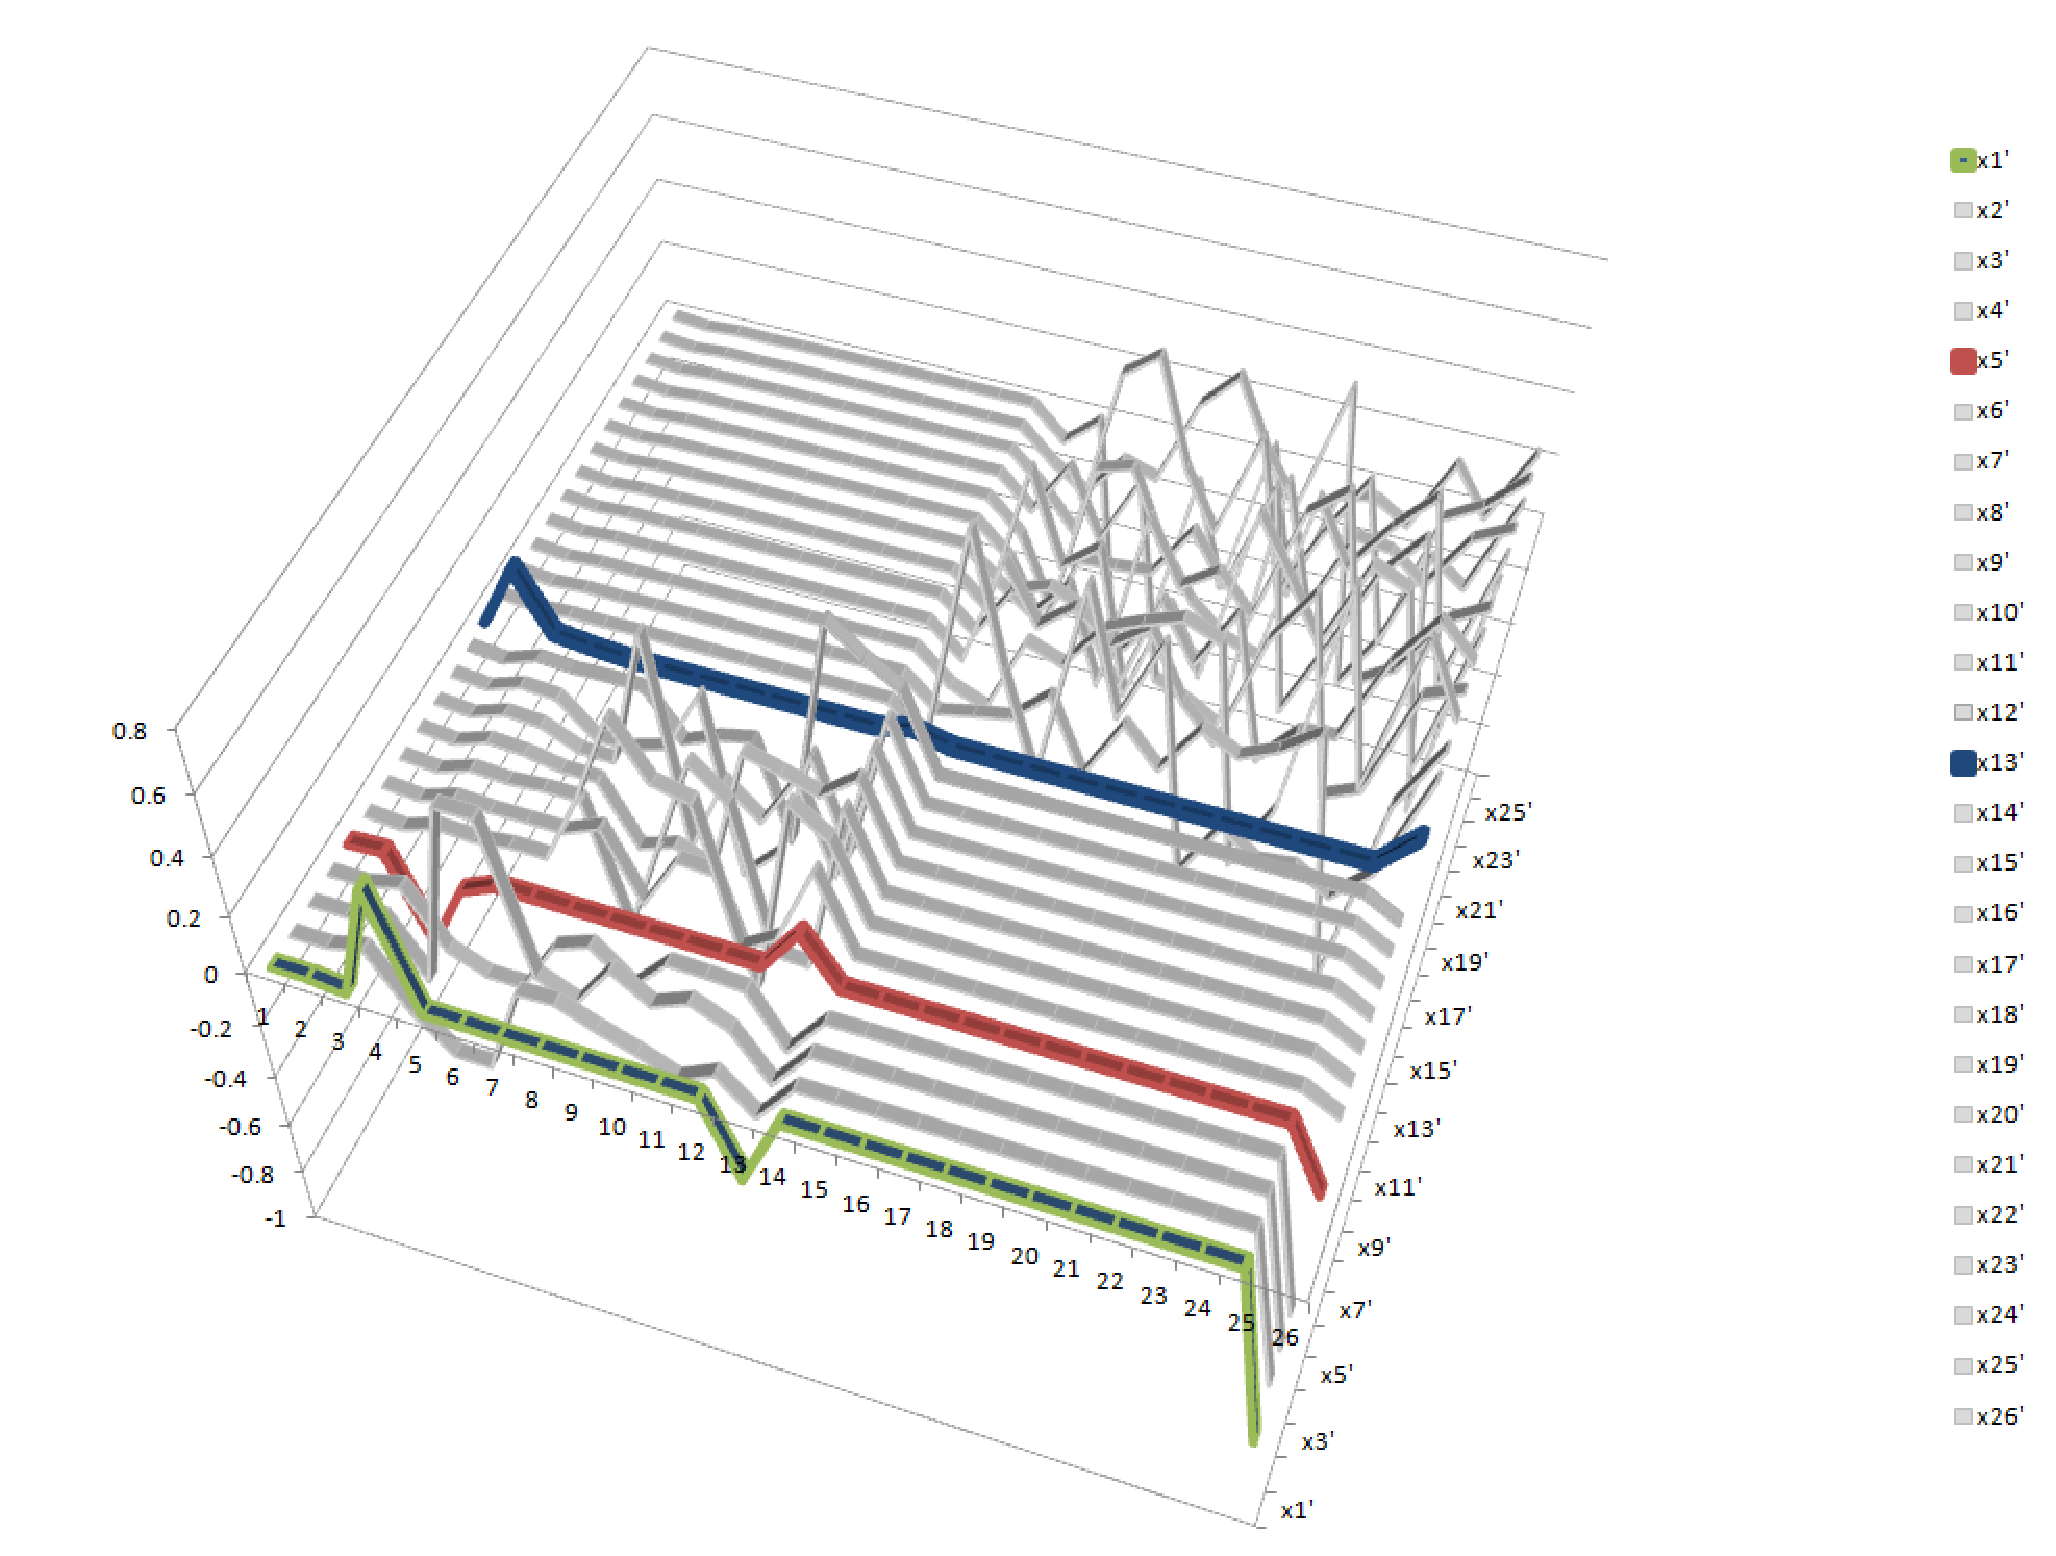
\includegraphics[width=.7\textwidth]{fig/embededNodeVectors.eps }
\caption[]{\label{fig:embededNodeVectors}.}
\end{figure}

\begin{figure}[tbh]
\centering
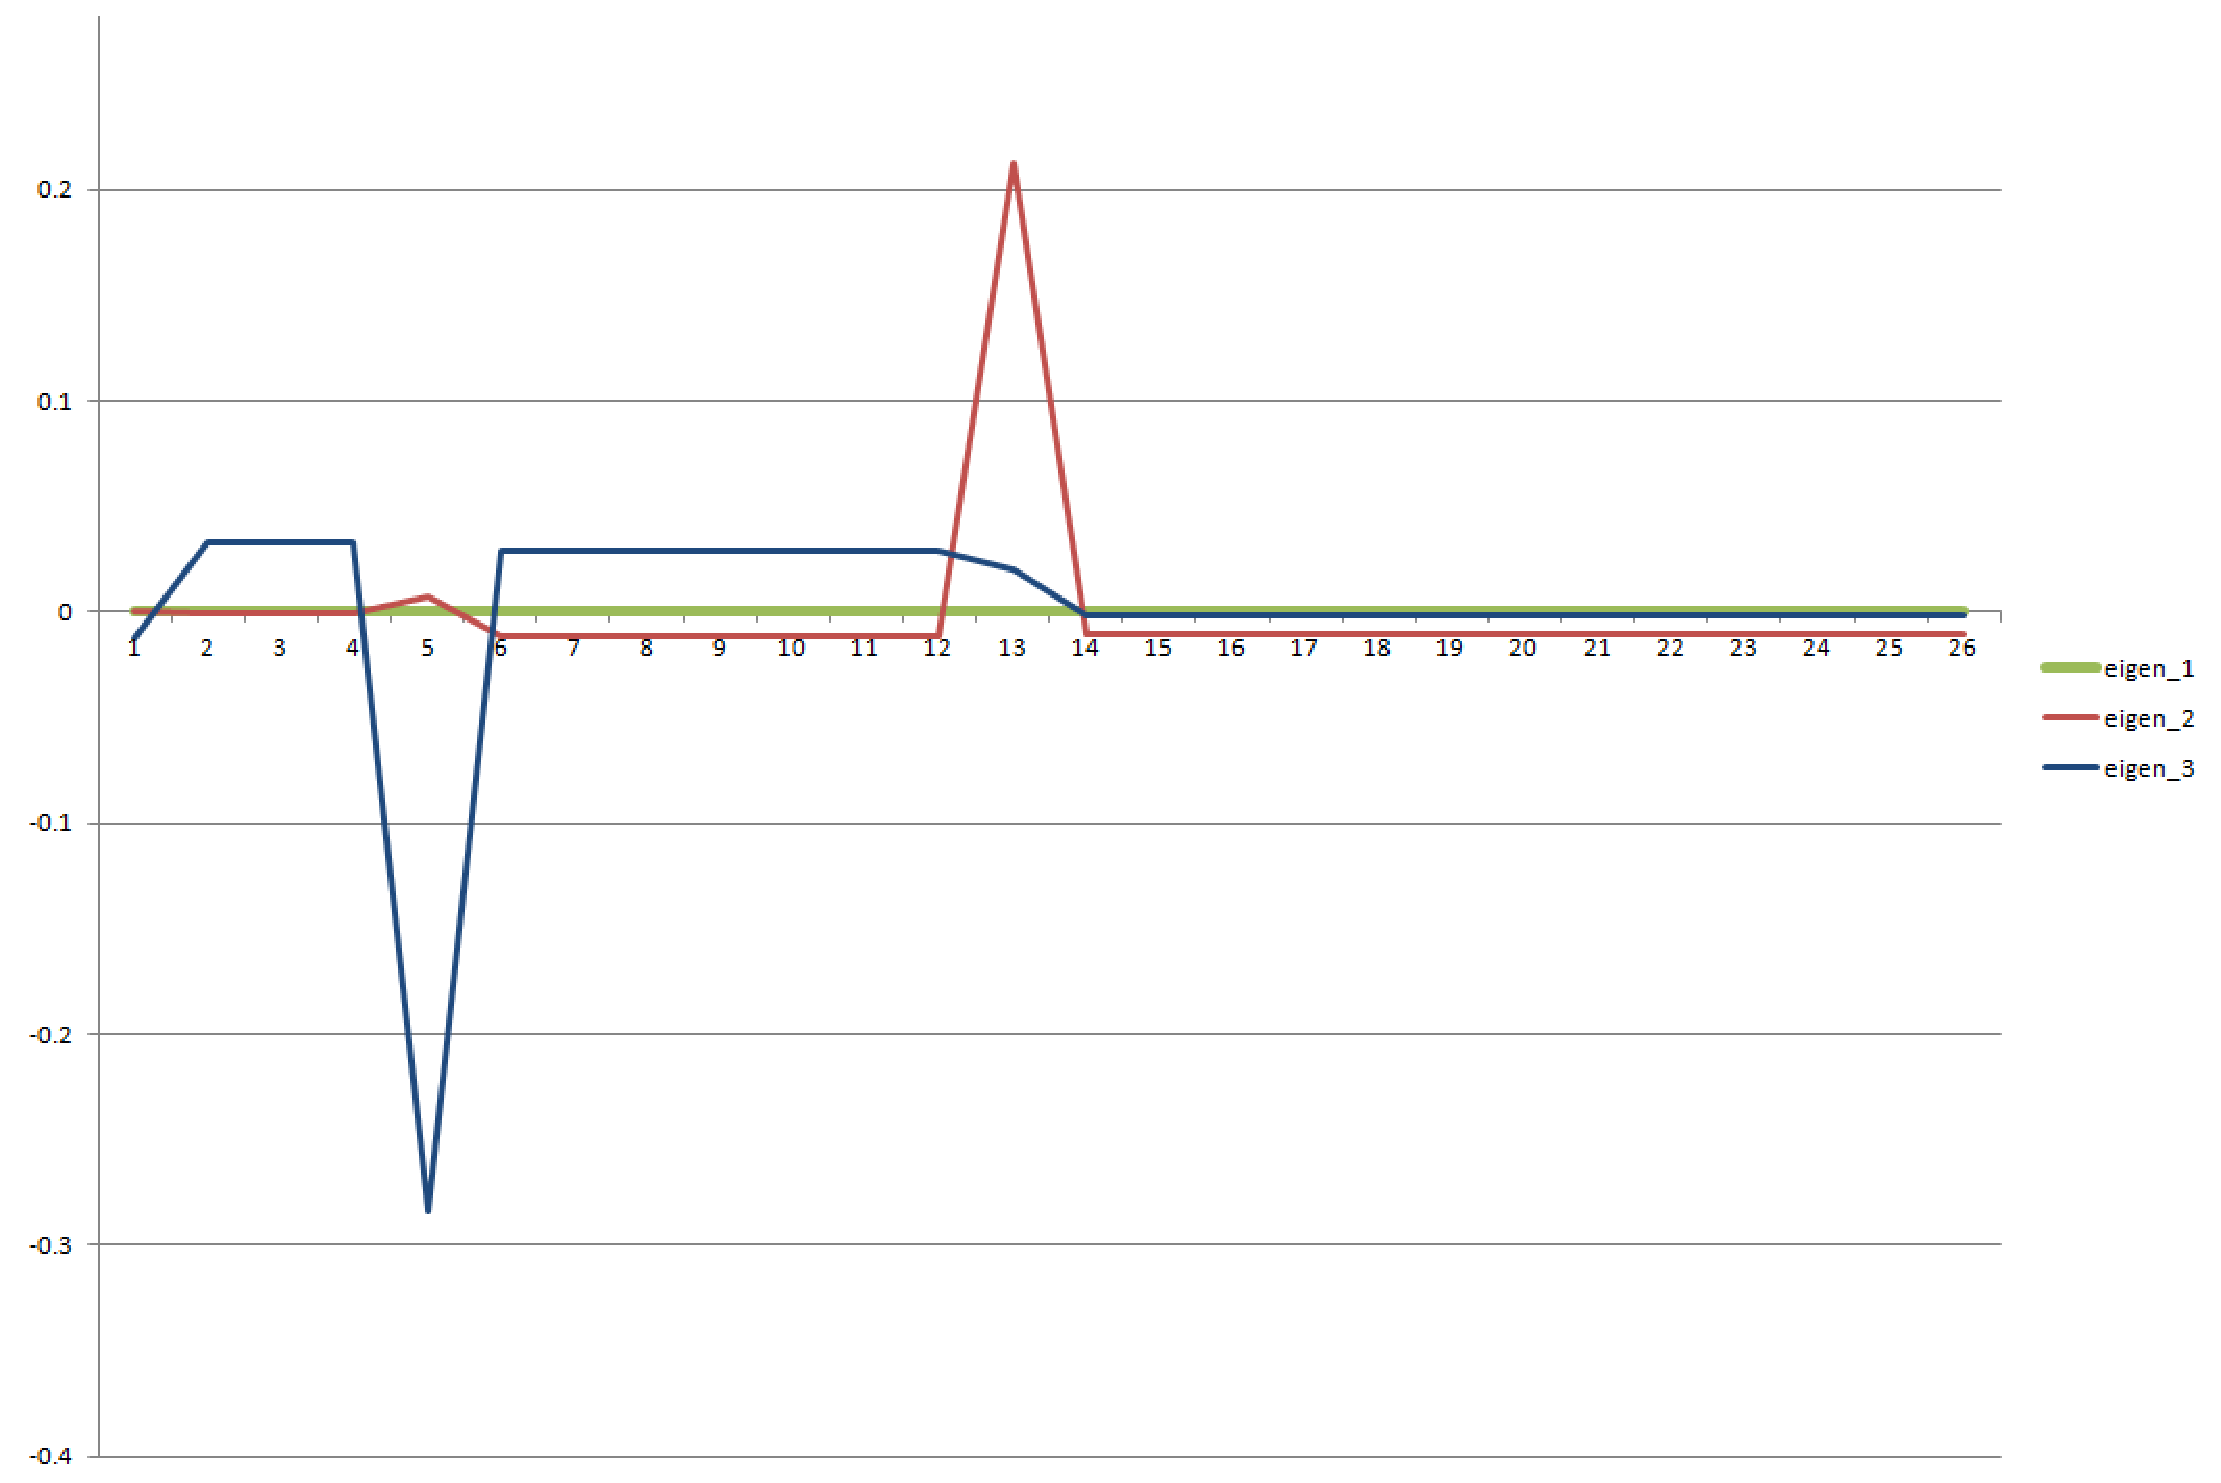
\includegraphics[width=.7\textwidth]{fig/eigens.eps }
\caption[]{\label{fig:eigens}.}
\end{figure}


%Similarly, with a movie database described below we find that the horror thriller Silence of the Lambs� to the children's film Free Willy have a smaller than average mutual commute time because both were box-office successes, yet the angle between them is larger than average because there was little overlap in their audiences.


For data that is relatively uniform (the out degree distribution of the graph does not follow a skewed distribution), the commute distance actually appears useful. However, for realistic data where the degree distribution follows a Zipf or power-law relationship, the commute distance displays a bias toward high degree nodes. This is due to the fact that high degree nodes will have a much higher stationary probability (probability that a random walk will be at the high degree node at any given time) and consequently all the distances are skewed toward the largest nodes.



\begin{figure}[tbh]
\centering
\begin{minipage}[c]{0.49\textwidth}\centering
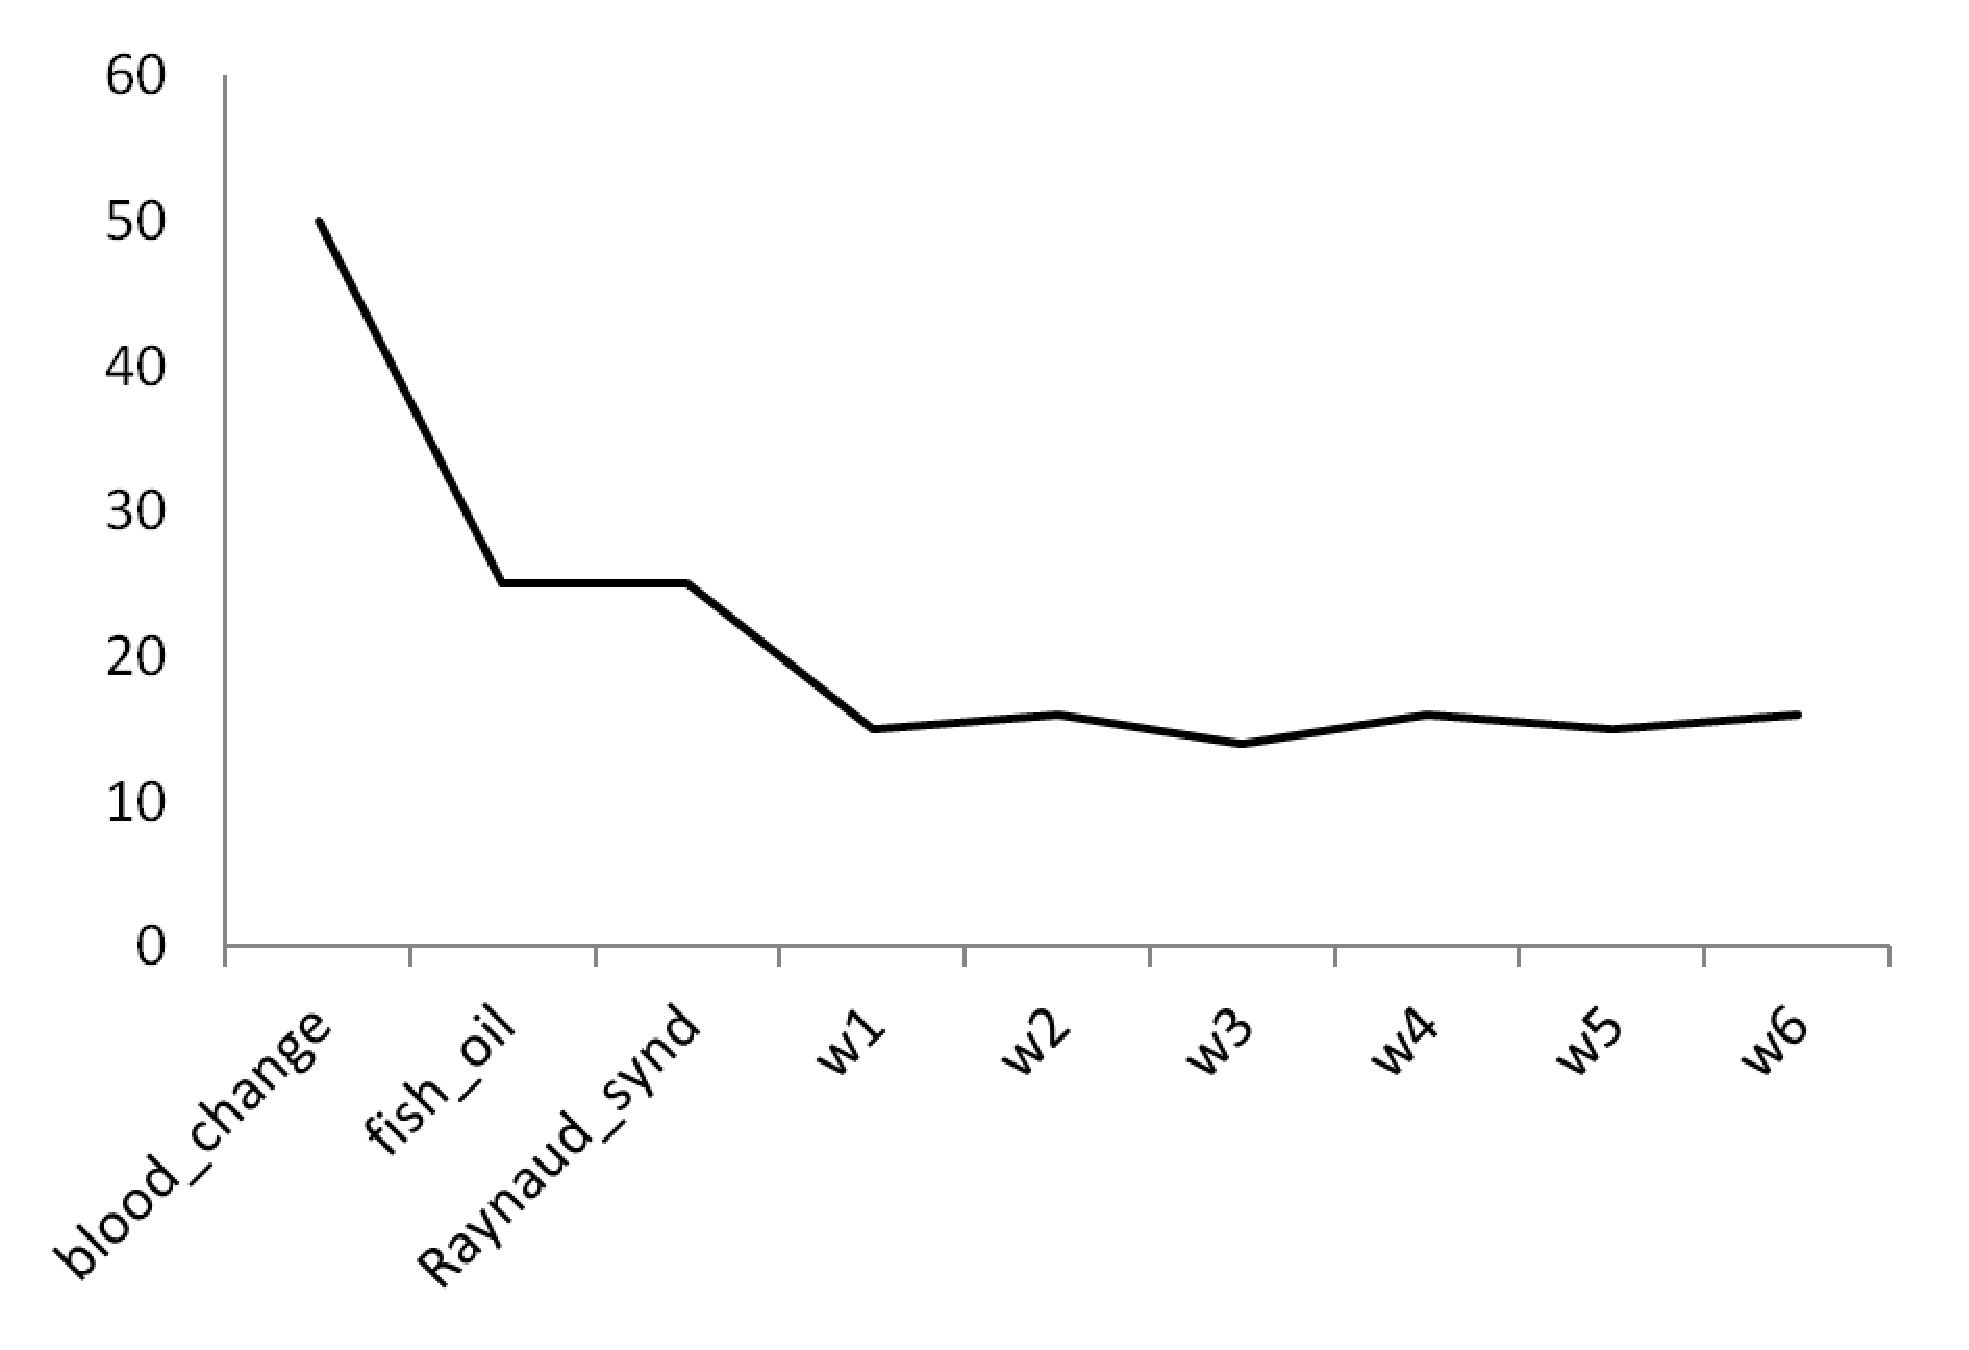
\includegraphics[width=\textwidth]{fig/distro-toy.eps}
\end{minipage}
\hfill
\begin{minipage}[c]{0.49\textwidth}\centering
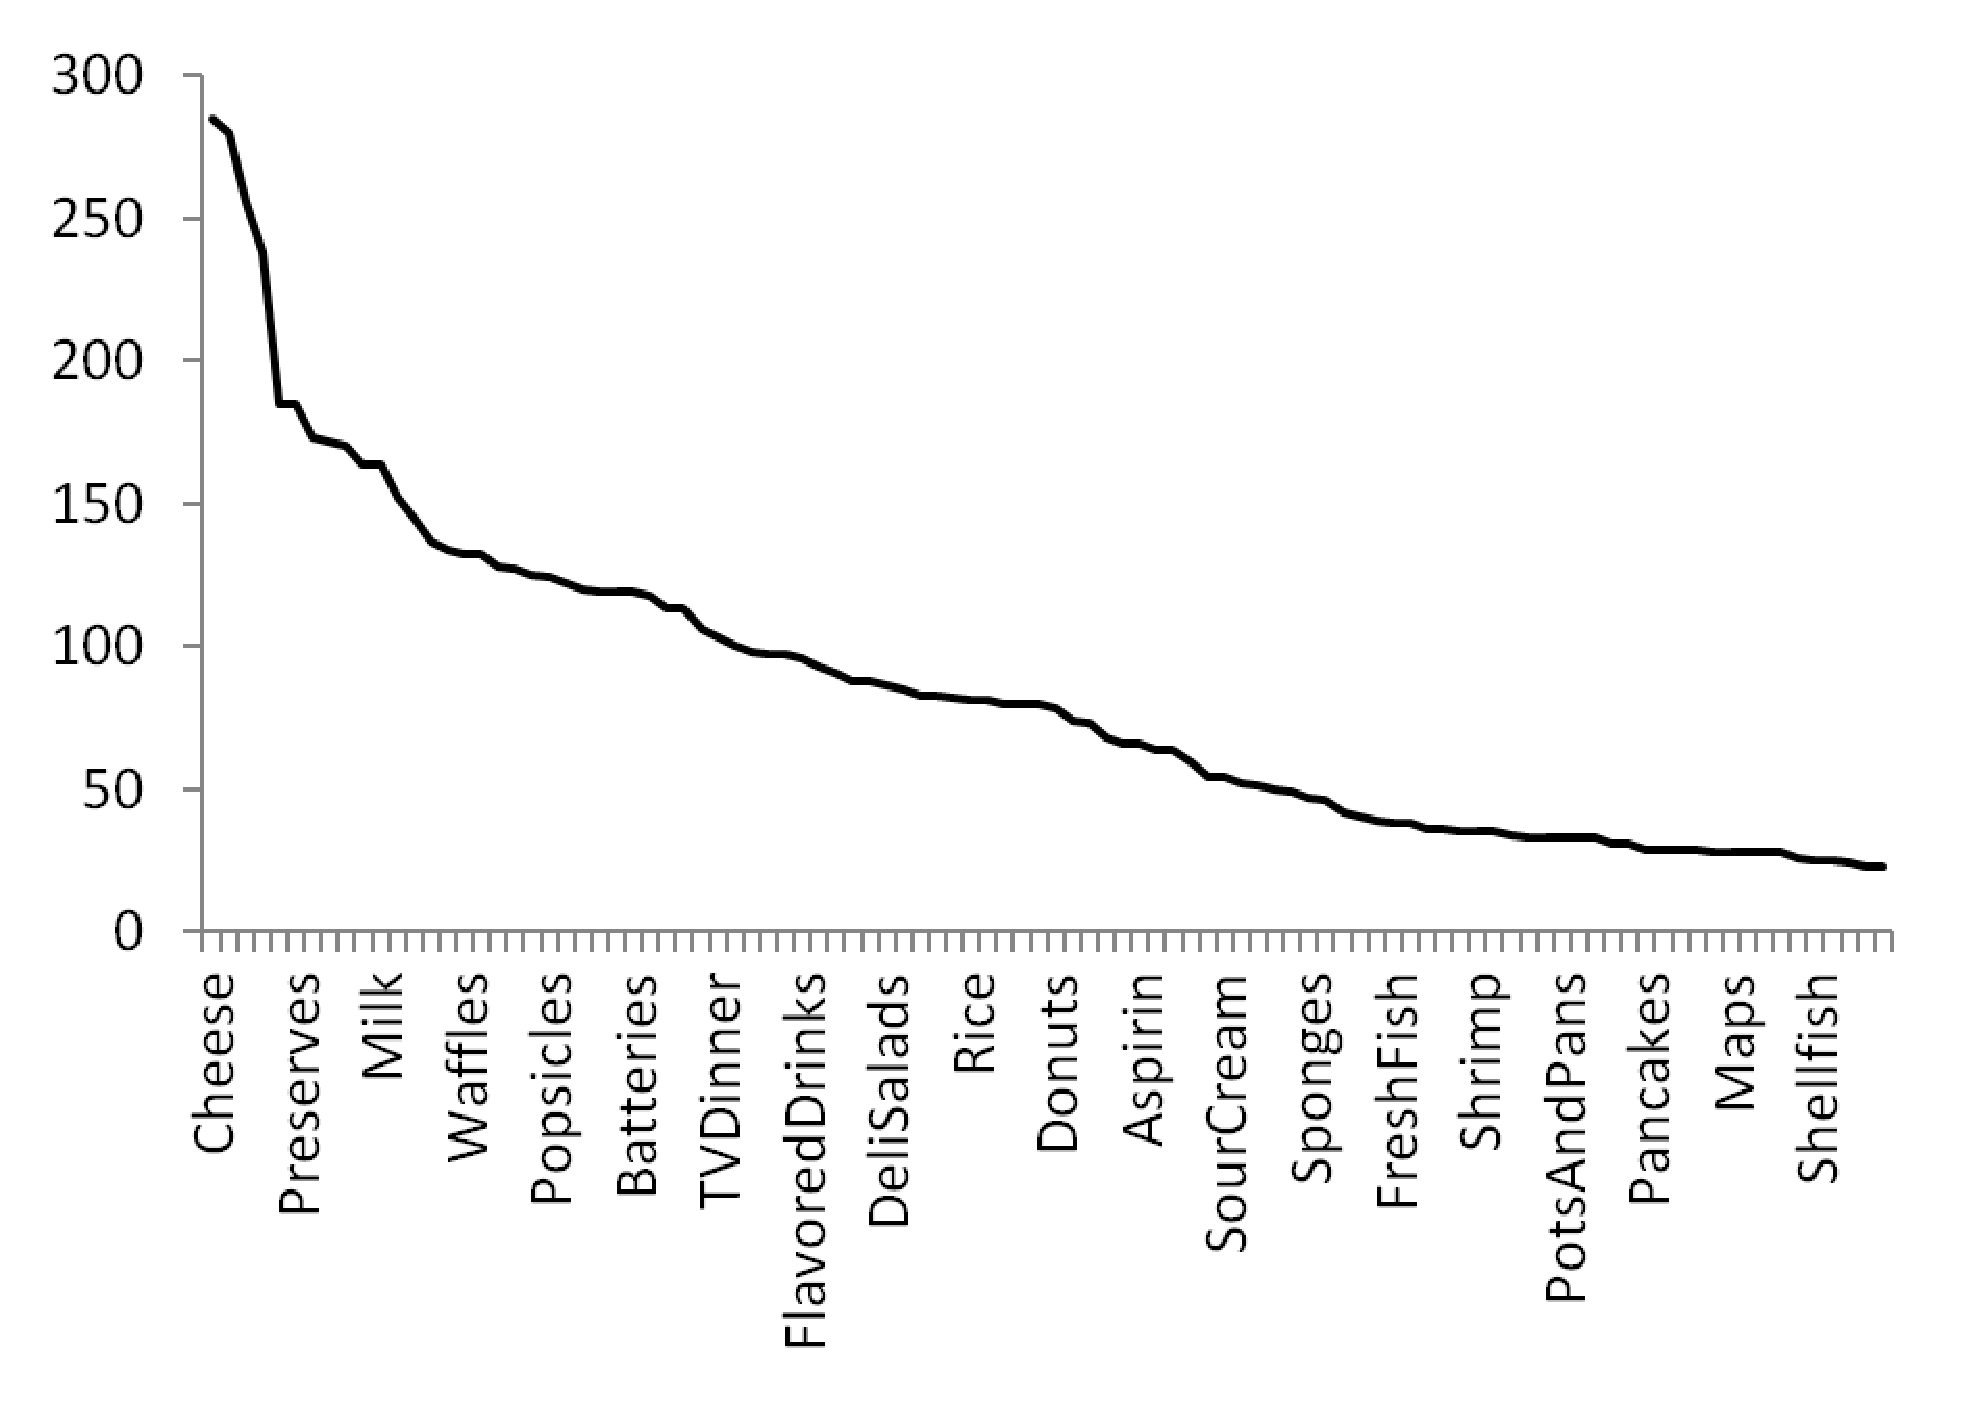
\includegraphics[width=\textwidth]{fig/distro-foodmart.eps}
\end{minipage}
\caption[]{\label{fig:distro}.}
\end{figure}

\begin{figure}[tbh]
\centering
\begin{minipage}[c]{0.49\textwidth}\centering
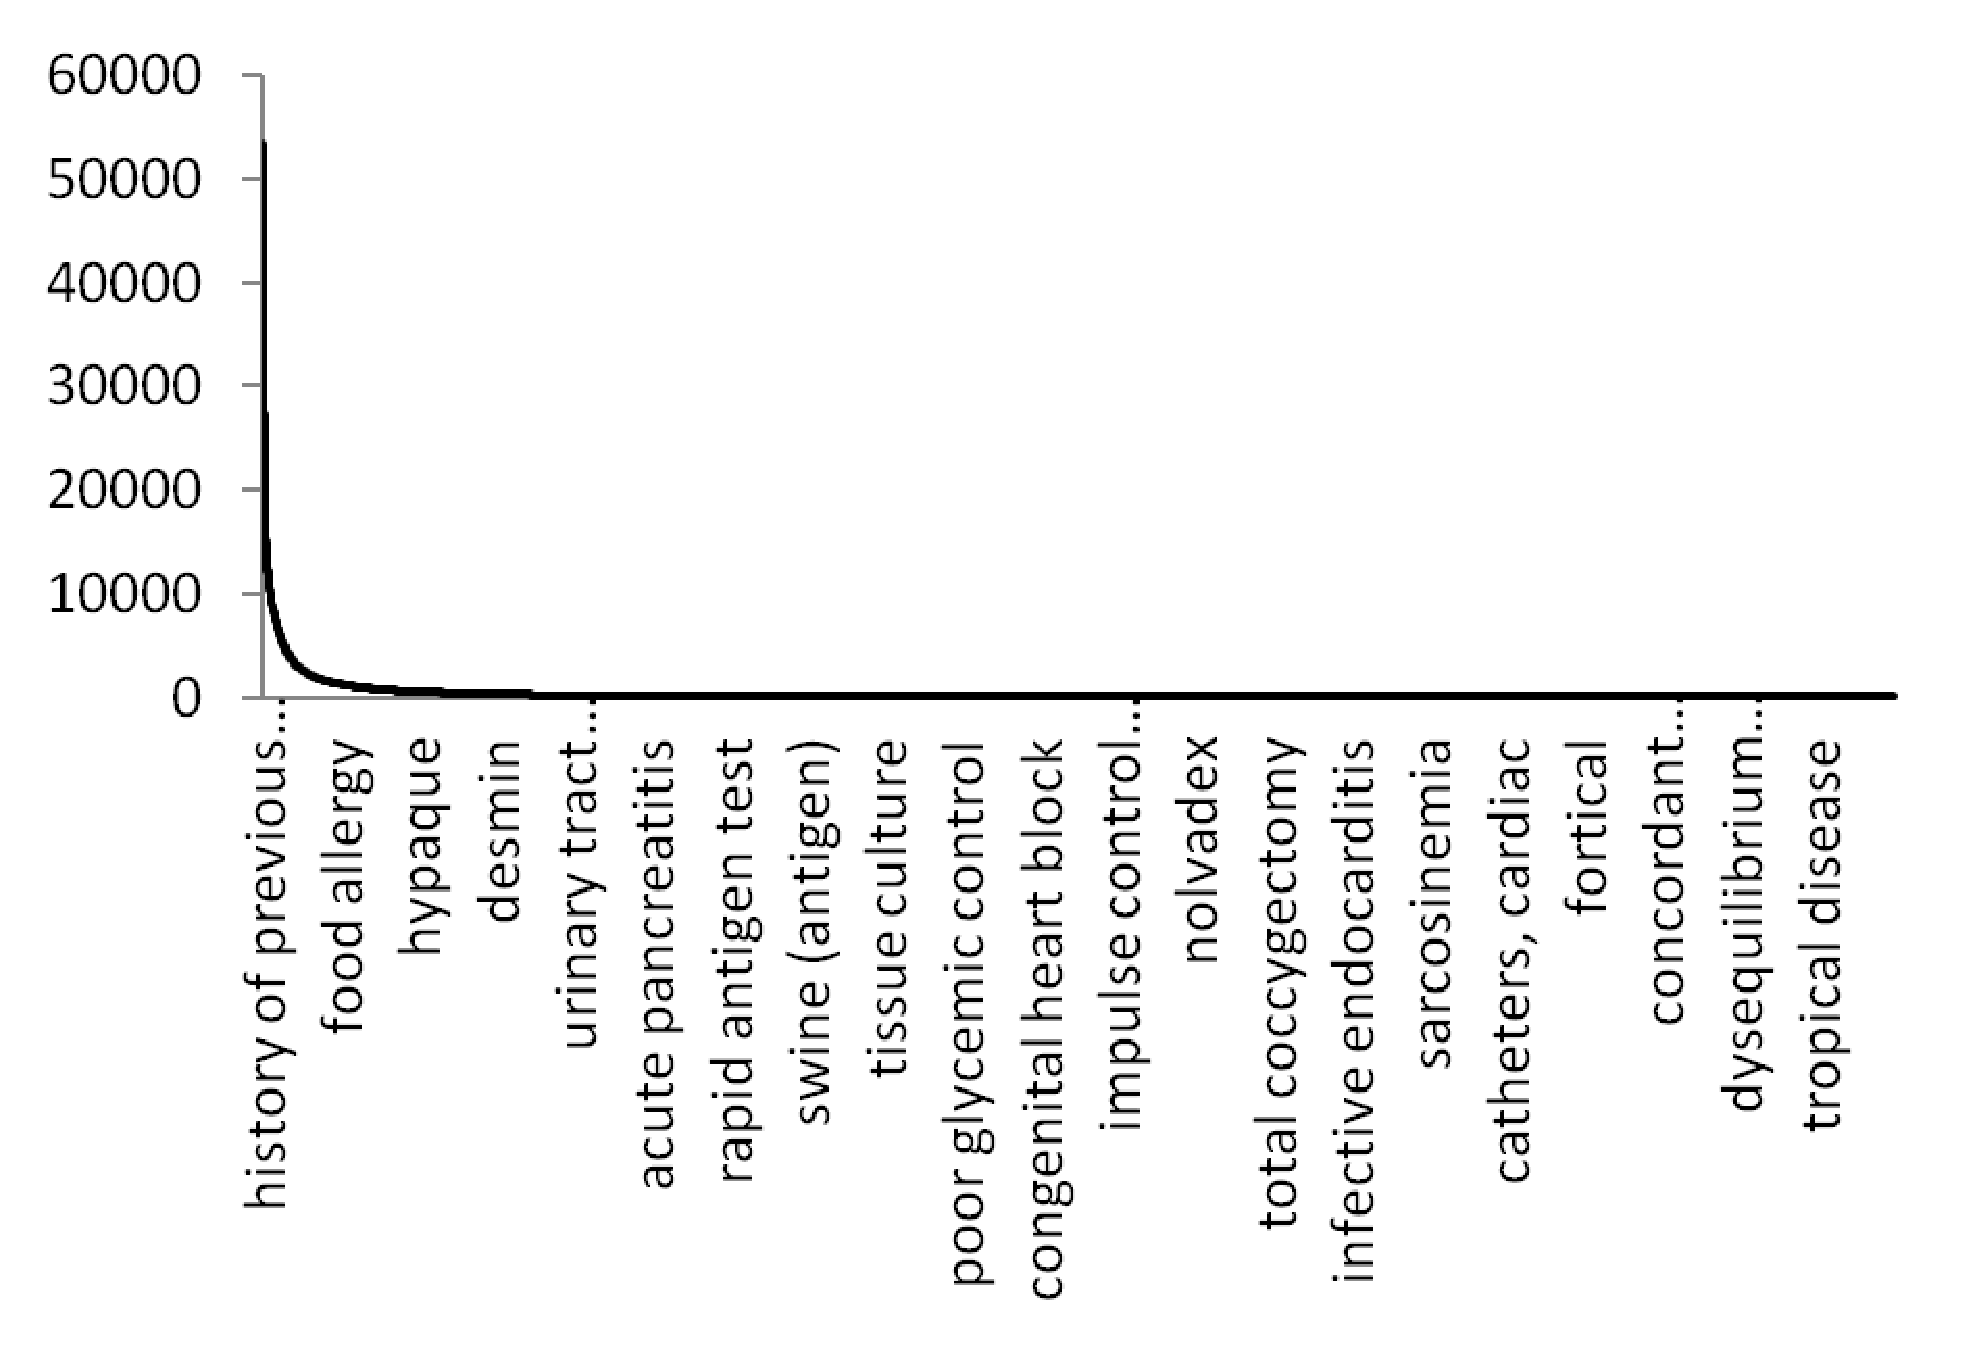
\includegraphics[width=\textwidth]{fig/distro-stride.eps}
\end{minipage}
\hfill
\begin{minipage}[c]{0.49\textwidth}\centering
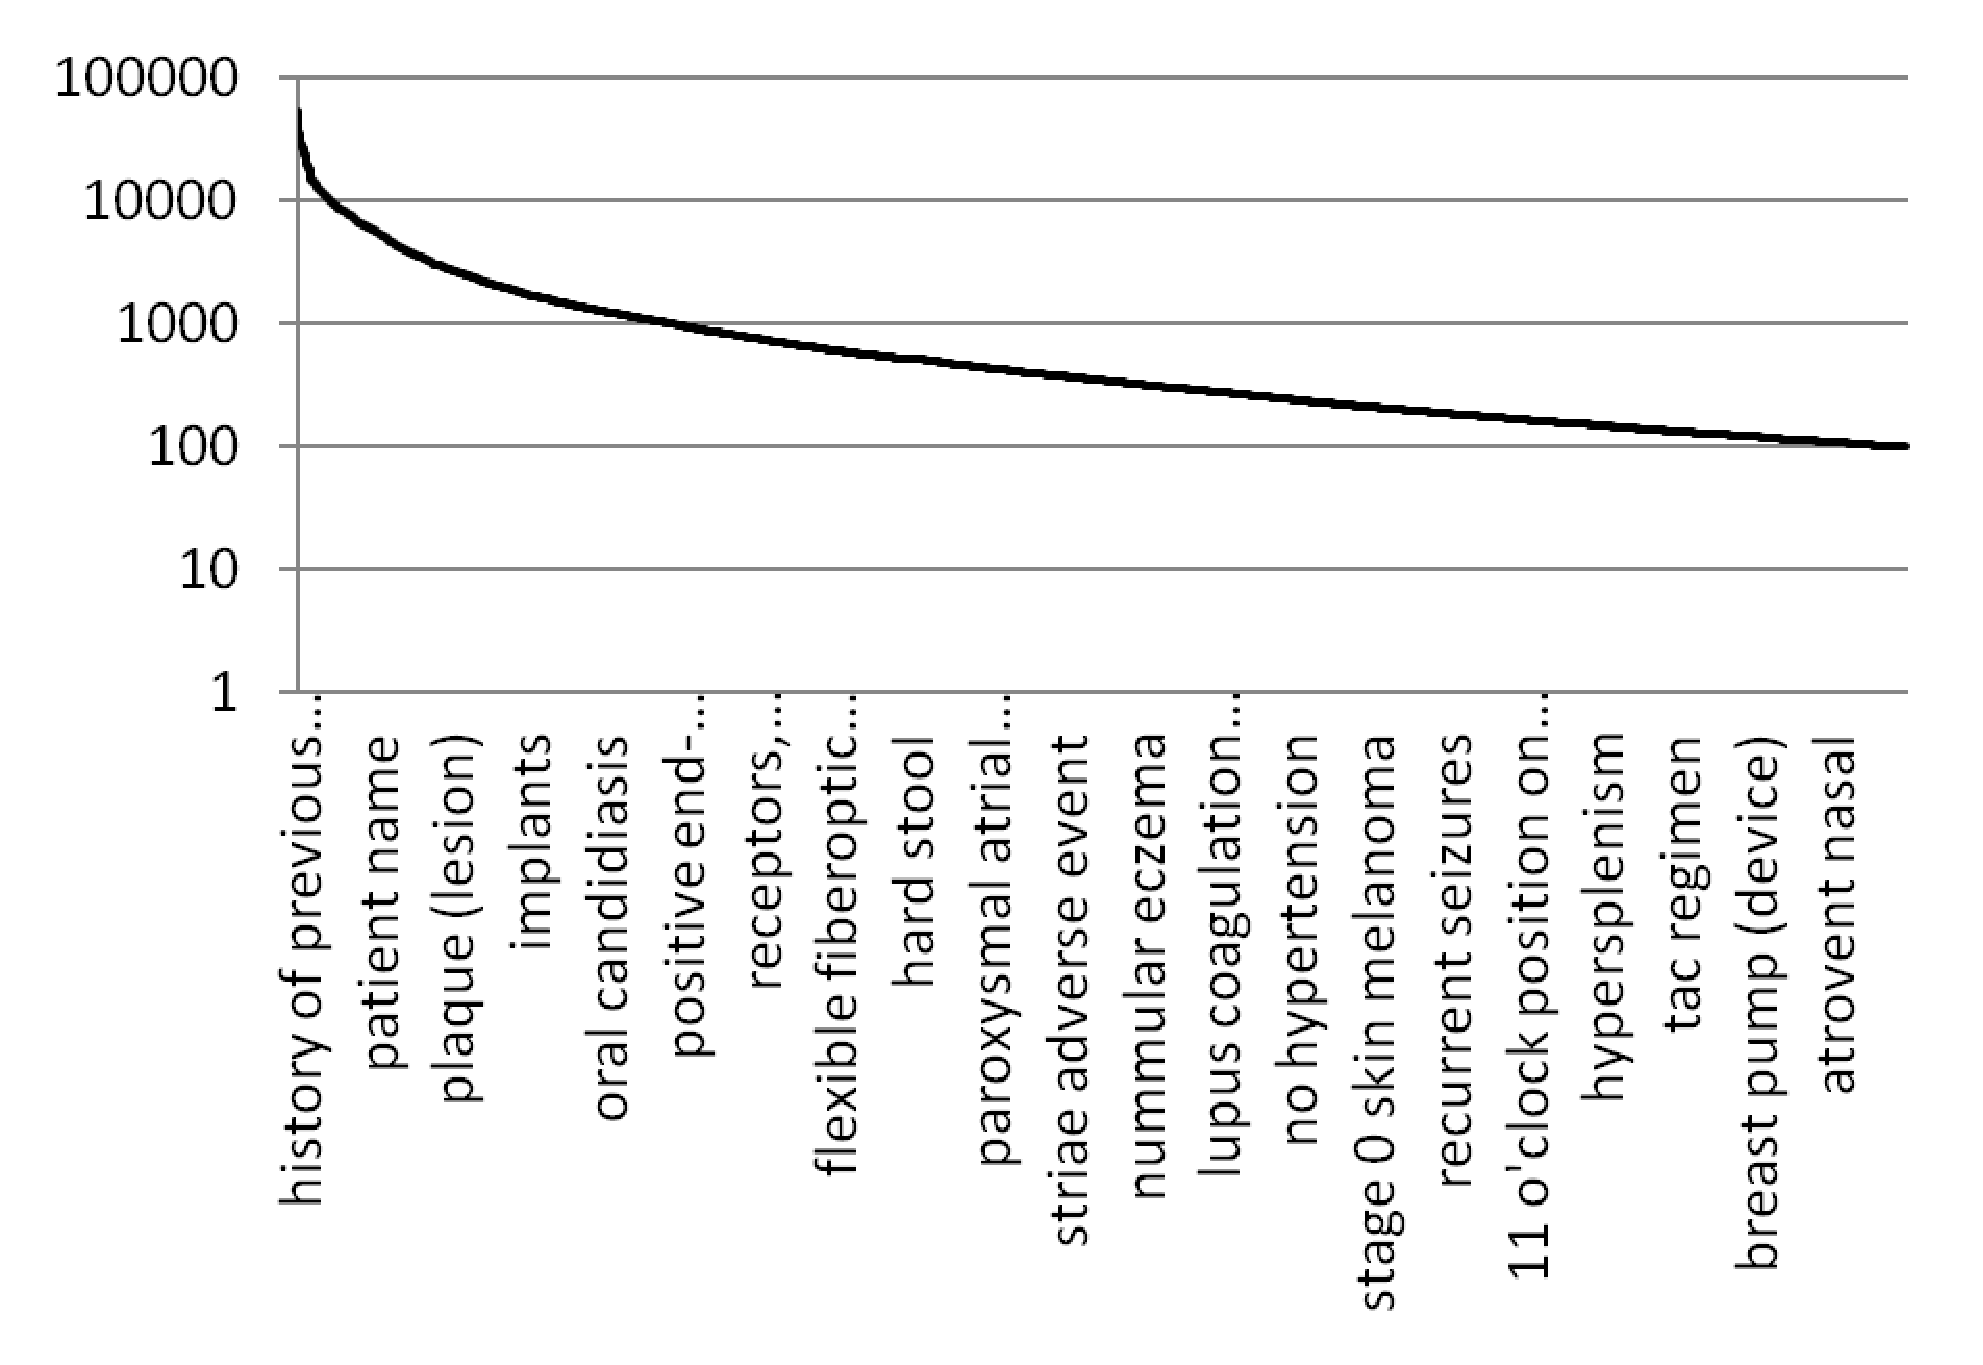
\includegraphics[width=\textwidth]{fig/distro-stride-log.eps}
\end{minipage}
\caption[]{\label{fig:distro2}.}
\end{figure}